\documentclass[12pt]{report}
\usepackage[utf8]{inputenc}
\usepackage[a4paper, margin=2.5cm]{geometry}
\usepackage{fancyhdr}
\usepackage[round]{natbib}
\usepackage{hyperref}
\usepackage{xcolor}
\usepackage{graphicx}
\usepackage[noend,ruled,vlined]{algorithm2e}
\usepackage{pdfpages}
\usepackage[acronym, nonumberlist]{glossaries}
\usepackage{minted}
\usepackage{subcaption}

\newcommand{\changefont}{%
    \bfseries\fontsize{8}{11}\selectfont
}
\fancyhf{}
\cfoot{\thepage}
\renewcommand{\headrulewidth}{0pt}
\fancyhead[R]{\changefont \nouppercase \rightmark} %section
\pagestyle{fancy}

\def\CCBY{\CCaux{by}{license/CCBY.png}{CC BY}}

\def\CCaux#1#2#3{%
\noindent\includegraphics[width=0.2\textwidth]{img/#2}\\{\textbf{\textsf{#3}}}
\\\url{https://creativecommons.org/licenses/#1/4.0/}\\}

\renewcommand{\baselinestretch}{1.5}

% Defining extra colors
\definecolor{dark-blue}{cmyk}{1.0,1.0,0.0,0.1}
\definecolor{dark-green}{cmyk}{1.0,0,1.0,0.4}
\definecolor{dark-red}{cmyk}{0,1.0,1.0,0.3}
\definecolor{navy-blue}{cmyk}{1.0,1.0,0.0,0.1}
\definecolor{grey}{rgb}{0.6,0.6,0.6}
\definecolor{eng}{cmyk}{0.14,0.71,1,0.03}
\definecolor{um}{cmyk}{0.25,1.00,1.00,0.22}
\definecolor{lightGray}{gray}{0.92}

\hypersetup{
%    bookmarks=true,						% show bookmarks bar?
	bookmarksnumbered=true,
	plainpages=false,					 	
    unicode=true,					 		% non-Latin characters in Acrobat’s bookmarks
    pdffitwindow=true,						% window fit to page when opened
    %pdfstartview={FitW},					% fits the width of the page to the window
    %pdftitle={My title},					% title
    pdfauthor={Rui Souto},		            % author
    %pdfsubject={Subject},					% subject of the document
    pdfcreator={Rui Souto},		            % creator of the document
    pdfproducer={Rui Souto},		        % producer of the document
    %pdfkeywords={keyword1} {key2} {key3},	% list of keywords
    %pdfnewwindow=true,						% links in new window
    colorlinks=true,						% false: boxed links; true: colored links
    linkcolor=dark-blue,					% color of internal links
    citecolor=dark-green,					% color of links to bibliography
    filecolor=magenta,						% color of file links
    urlcolor=navy-blue						% color of external links
}

\makeglossaries
\loadglsentries{glossaries}

\begin{document}

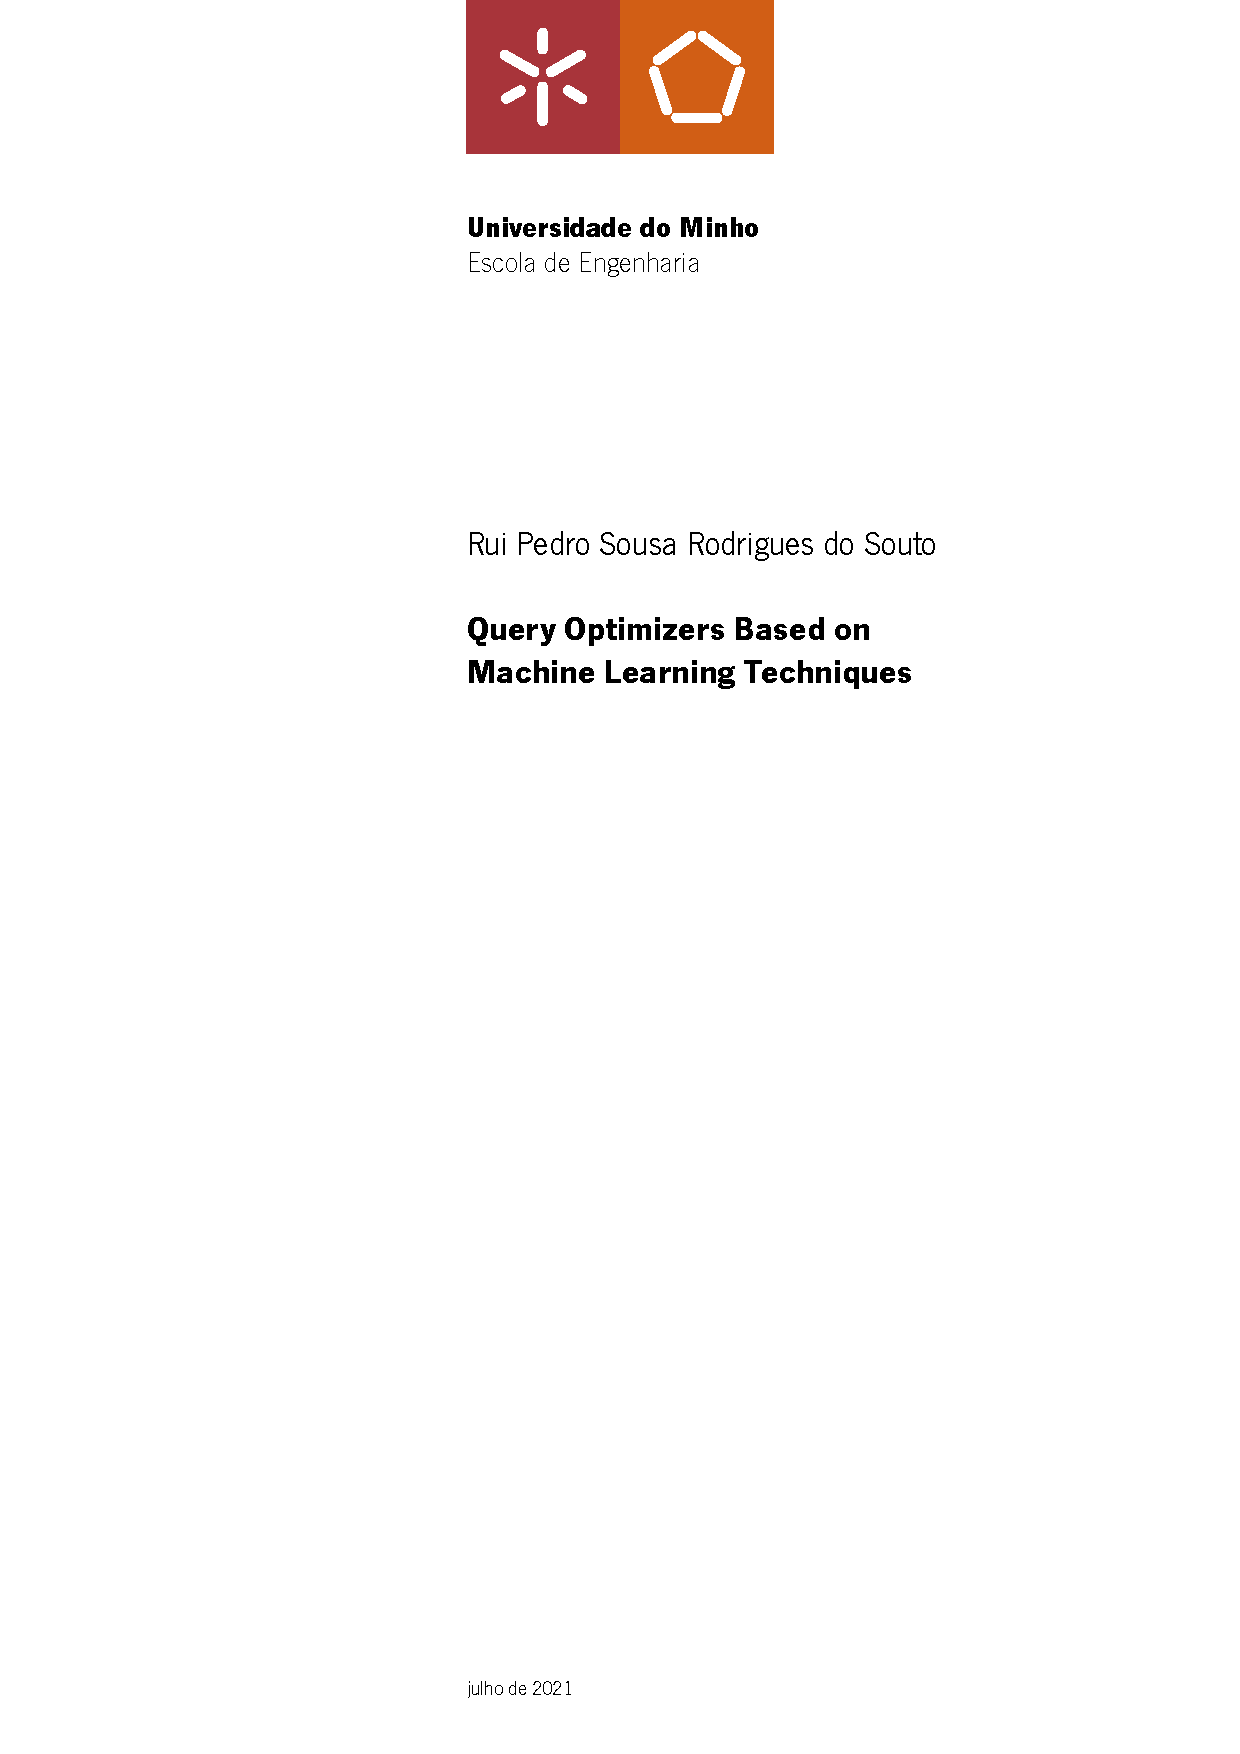
\includepdf{cover/frontcover_2.pdf}
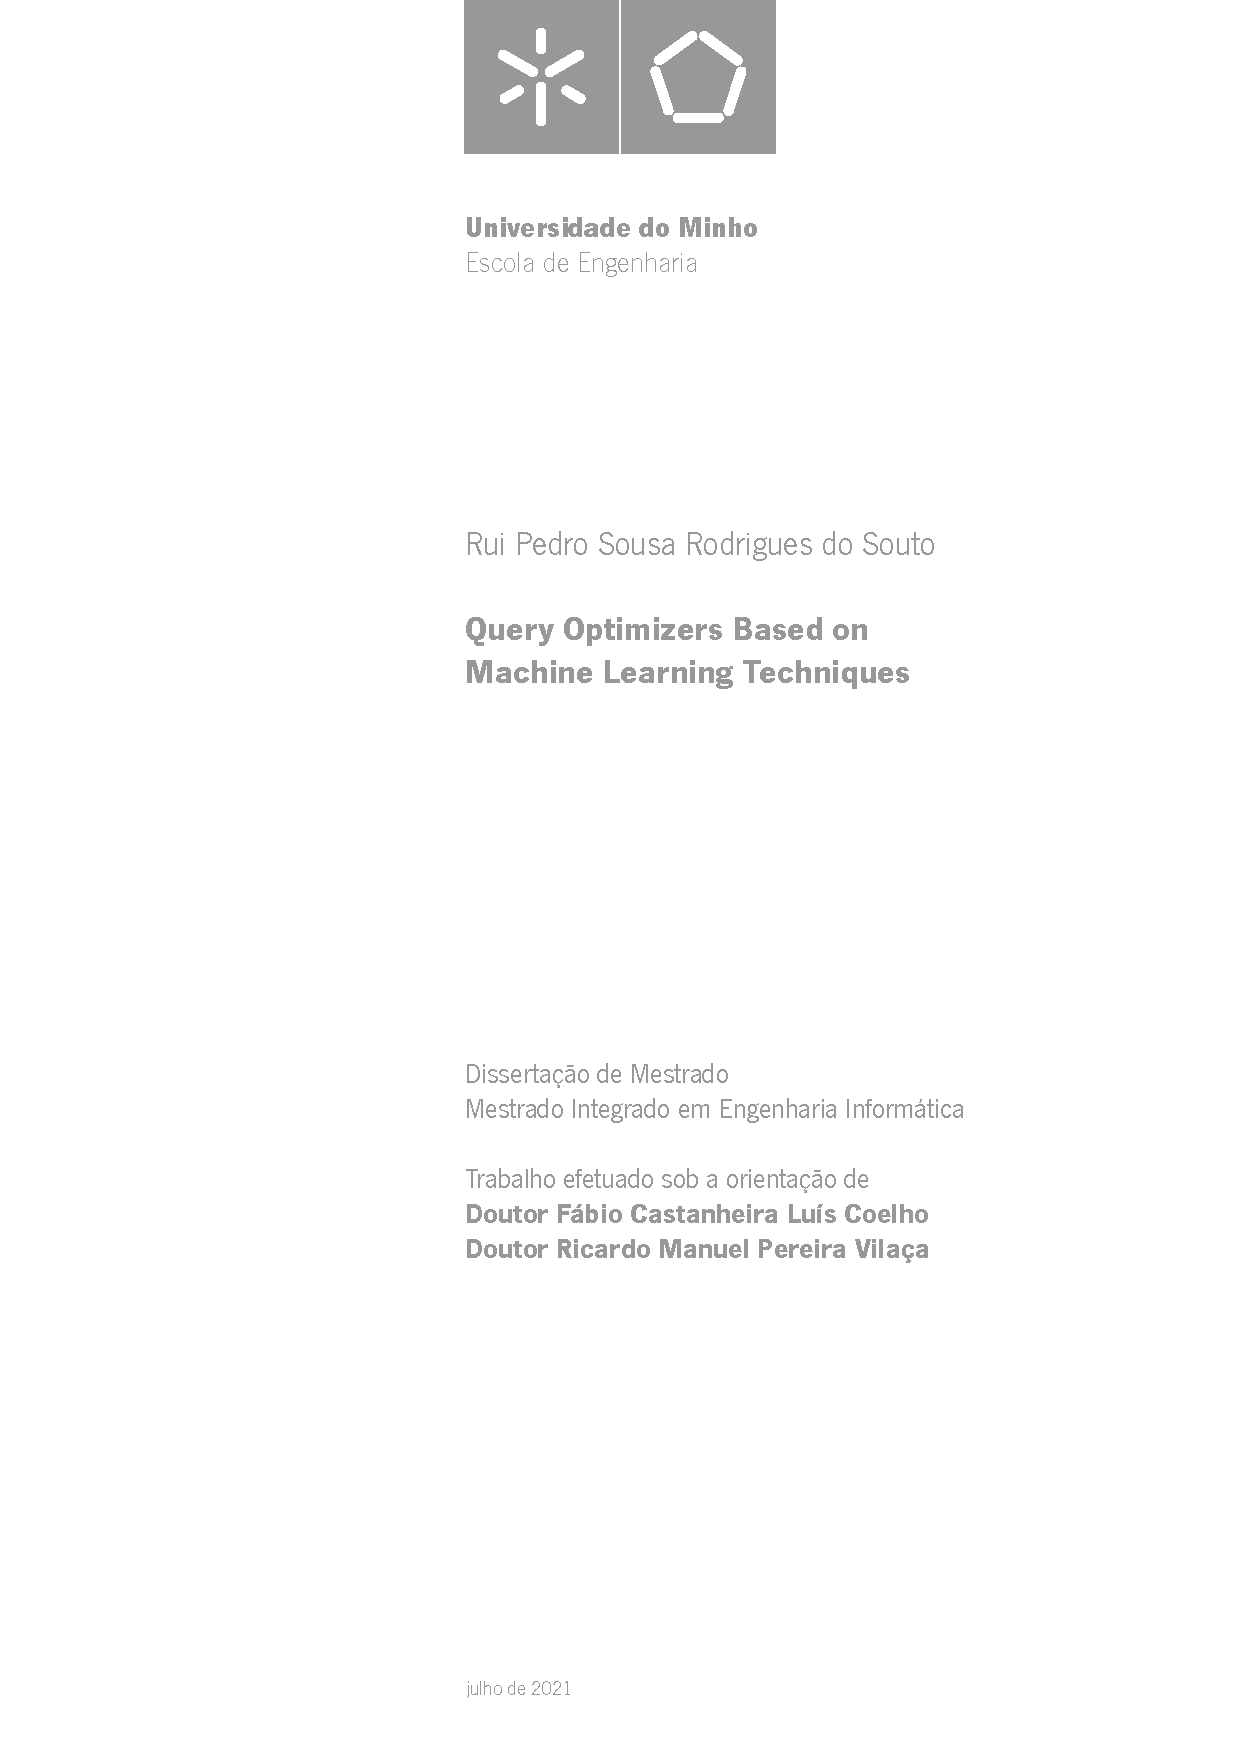
\includepdf{cover/backcover.pdf}

\pagenumbering{roman}
\setcounter{page}{1}

\chapter*{Copyright and Terms of Use for Third Party Work}

    \noindent This dissertation reports on academic work that can be used by third parties as long as the internationally accepted standards and good practices are respected concerning copyright and related rights.

\vskip 1em
\noindent This work can thereafter be used under the terms established in the license below.
\vskip 1em

\noindent Readers needing authorization conditions not provided for in the indicated licensing should contact the author through the RepositóriUM of the University of Minho.

\vskip 1em
\noindent \textbf{\textit{License granted to users of this work}}
\vskip 1em

\CCBY

\chapter*{Acknowledgments}

    Throughout the writing of this dissertation, I have received a great deal of support and assistance.

I would like to express my deep gratitude to Fábio Coelho and Ricardo Vilaça, my research supervisors. Without your assistance and dedicated involvement in every step throughout the process, this dissertation would not have been possible, and you brought this work to a higher level.

I would like to extend my sincere thanks to every member of High-Assurance Software Laboratory (HASLab) \& INESC TEC for all their help. You provided me with the tools that I needed to choose the right direction and successfully complete my dissertation.

I would like to express my profound gratitude to my family for investing in my education and always providing me everything I needed to strive, without which none of this work or the previous five years would have been possible. You are always there for me.

Some special words of gratitude go to all my friends who have always been a major
source of support when things would get a bit discouraging. The last few years would have been unthinkable without all of the stories we have shared and all the help you have provided.

The last word goes for my loved one, Mariana, whose invaluable and unconditional support was what kept me moving. Every time I was ready to quit, you did not let me, and I am forever grateful. This dissertation stands as a testament to your unfailing support and continuous encouragement.

\bigbreak
\hfill \textit{Thank you}
\bigbreak

%Fabio: Incluir esta referência para o financiamento Não esquecer o agradecimento ao INESC TEC e ao HASLab

This work is financed by National Funds through the Portuguese funding agency, FCT - Fundação
para a Ciência e a Tecnologia, within project UIDB/50014/2020.

\chapter*{Statement of Integrity}

    I hereby declare having conducted this academic work with integrity.

\vskip 1em
\noindent I confirm that I have not used plagiarism or any form of undue use of information or falsification of results along the process leading to its elaboration. 
\vskip 1em

\noindent I further declare that I have fully acknowledged the Code of Ethical Conduct of the University of Minho.

\chapter*{Abstract}

    Query optimizers are considered one of the most relevant and sophisticated components in a database management system. However, despite currently producing nearly optimal results, optimizers rely on statistical estimates and heuristics to reduce the search space of alternative execution plans for a single query. As a result, for more complex queries, errors may grow exponentially, often translating into sub-optimal plans resulting in less than ideal performance. Recent advances in machine learning techniques have opened new opportunities for many of the existing problems related to system optimization. 

This document proposes a solution built on top of PostgreSQL that learns to select the most efficient set of optimizer strategy settings for a particular query. Instead of depending entirely on the optimizer's estimates to compare different plans under different configurations, it relies on a greedy selection algorithm that supports several types of predictive modeling techniques, from more traditional modeling techniques to a deep learning approach.

The system is evaluated experimentally with the standard \gls{tpch} and Join Ordering Benchmark workloads to measure the cost and benefits of adding machine learning capabilities to traditional query optimizers.

\paragraph{Keywords} Database tuning, machine learning, query optimization
    
\chapter*{Resumo}

    Os otimizadores de \textit{queries} são considerados um dos componentes de maior relevância e complexidade num sistema de gestão de bases de dados. No entanto, apesar de atualmente produzirem resultados quase ótimos, os otimizadores dependem do uso de estimativas estatísticas e de heurísticas para reduzir o espaço de procura de planos de execução alternativos para uma determinada \textit{query}. Como resultado, para \textit{queries} mais complexas, os erros podem crescer exponencialmente, o que geralmente se traduz em planos sub-ótimos, resultando num desempenho inferior ao ideal. Os recentes avanços nas técnicas de aprendizagem automática abriram novas oportunidades para muitos dos problemas existentes relacionados com otimização de sistemas.

Este documento propõe uma solução construída sobre o PostgreSQL que aprende a selecionar o conjunto mais eficiente de configurações do otimizador para uma determinada \textit{query}. Em vez de depender inteiramente de estimativas do otimizador para comparar planos de configurações diferentes, a solução baseia-se num algoritmo de seleção \textit{greedy} que suporta vários tipos de técnicas de modelagem preditiva, desde técnicas mais tradicionais a uma abordagem de \textit{deep learning}.

O sistema é avaliado experimentalmente com os \textit{workloads} \gls{tpch} e Join Ordering Benchmark para medir o custo e os benefícios de adicionar aprendizagem automática a otimizadores de \textit{queries} tradicionais.

\paragraph{Palavras-chave} Aprendizagem automática, otimização de \textit{queries}, \textit{tuning} de base de dados
    
\cleardoublepage
\tableofcontents

\cleardoublepage
\addcontentsline{toc}{chapter}{\listfigurename}
\listoffigures
	
\cleardoublepage
\addcontentsline{toc}{chapter}{\listtablename}
\listoftables

\cleardoublepage
\printglossaries
\addcontentsline{toc}{chapter}{Glossary}

\cleardoublepage
\pagenumbering{arabic}
\setcounter{page}{1}
    
\chapter{Introduction}

    The amount of generated data is currently growing exponentially. As a result, relational database management systems continue to be the most widely used solution in business environments to support transactional data storage. Such systems store information in the form of tables, where data is stored in rows and columns.

The widespread use of relational databases is partly due to the use of declarative data query languages (i.e., \gls{sql}). The abstraction from the actual low-level details of the physical organization of data allows complex queries to be expressed concisely and straightforwardly while providing a lot of querying flexibility. For this reason, the user only needs to specify the form of the result to be obtained and not the procedure to achieve it.

The query processor is the module that reads the query and generates the low-level procedure that should be executed to obtain the result. It starts by transforming the user-declared query into a lower-level relational algebra representation that outlines an efficient execution plan.

An important aspect of query processing is optimization. During this process, the query is optimized, and the most efficient plan among the different possible strategies that can be used to process it is selected. Since users are not expected to write queries as efficiently as possible, it is up to the system to build an execution plan that minimizes their execution cost. Usually, this process includes three separate components: search space, cost model, and search strategy. The search space is the set of alternative execution plans that return the same result and is obtained by applying transformation rules at the relational algebra level. They vary in how the operations involved are conducted and how they are implemented, resulting in different performance levels. The cost model tries to estimate the cost of a single execution plan. Finally, the search strategy exploits the search space to choose the plan that maximizes performance based on cost model predictions.

%Although this entire process takes place in centralized and distributed environments, it is much more complex in distributed database systems as more factors interfere with performance. Additionally, the relations involved in a particular query may be fragmented and replicated, adding communication costs to the equation.

In recent years, we have witnessed the exponential growth in the study and development of machine learning applications in systems' optimization. It has opened different possibilities of applying machine learning techniques in the architecture of database systems, which are becoming increasingly complex and hard to tune. This dissertation studies the practicality and utility of sophisticated machine learning techniques regarding query optimization as a promising approach.

    \section{Problem}
    	Query optimization is the link between declarative languages and the efficient execution of queries expressed in them. However, it is essential to state that no optimizer generates optimal plans \citep{Bailis2015}. First, the cost of a particular plan is obtained by considering statistical information about the relations expressed in the query. There is a trade-off between the accuracy of these statistics and their maintenance costs, as more accurate statistics are significantly harder to maintain. For this reason, all optimizers rely on cardinality estimates that are usually measured based on simplifying assumptions such as uniformity and independence \citep{Leis2015}. Such assumptions are often incorrect in real-world data sets, leading to sub-optimal and sometimes disastrous plans.

Furthermore, exploiting a very large search space may have a higher computational cost than the runtime itself and is considered a NP-hard problem. This is why optimizers employ a set of heuristics to limit the size of their search space. The fact that query optimization still relies on carefully tuned and complex heuristics that have been designed over the years means that they require even more tuning by expert database administrators to improve query performance on each database. Additionally, even if using these heuristics is an effective way of restricting the search space, in some cases, they can fall short, resulting in bad plans \citep{Leis2015}.

    
    \section{Contributions}
        Intending to address current query optimization limitations of relational databases, this document describes the design and implementation of a proof-of-concept to provide machine learning capabilities to conventional database systems. At a high level, Odin implements predictive modeling techniques to guide a traditional query optimizer and select the execution strategy the query optimizer should use for that query, limiting and steering the search space. To achieve this, the approach relies on the availability of historical query execution data to generate predictive models and estimate the cost of executing alternative plans, each generated under different optimizer configurations.

The proposed solution improves the system's decision-making process, making it more dynamic and adaptive instead of relying entirely on a complex set of heuristics and statistical estimates. In addition, it does not replace or discard the query optimizer completely but instead adopts procedures readily available in most relational database systems and works in tandem with the query optimizer to improve query runtime. Finally, it provides a flexible, embedded, and extensible architecture supporting new data sources and query processing and optimization approaches. 
        
    \section{Document Structure}
        The rest of the document is organized in the following manner: Chapter 2 addresses state of the art and concepts of interest to provide a better framing of the work as well as discussion of the guiding principles considered during its development; Chapter 3 details the solution, beginning with a high-level architecture overview and followed by an explanation of each developed module; Chapter 4 presents an analysis and discussion of the results obtained during the experimental evaluation, describing experimental setups, workloads, metrics, and results; Finally, Chapter 5 outlines the main conclusions and deductions obtained from the experimental evaluation, followed by a proposal of the directions this work could take in the future.

\chapter{State of the Art}

    This chapter introduces the relevant state of the art to this dissertation. Currently, relational database management systems rely on a vast number of query optimization techniques that were continuously developed and implemented into production systems over several decades.

First, an introduction to query processing is given, discussing the basic concepts and strategies for optimizing queries. It starts by characterizing the main components involved in the process and the standard algorithm used to enumerate semantically equivalent plan alternatives. Finally, dynamic query optimization techniques are discussed.

Moreover, an overview of the broad domain of machine learning is provided, describing its fundamental concepts, multiple paradigms, types of tasks, and different machine learning algorithms.

The final section narrows the gap between machine learning and optimization of database systems. It discusses possible courses of action and describes the relevant related work concerning machine learning techniques in database systems. In the end, based on the analysis of related work, a discussion around the limitations of the current solutions is presented as well as the guiding principles that are taken into consideration during the development of the proposed solution.
    
    \section{Foundations of Query Processing}
    
        \label{sec:foundations_of_query_processing}

There is considerable work in database systems, from architectures and techniques for transaction and query processing to data models, languages, and user interfaces. This section focuses primarily on query processing and gives a comprehensive overview of what techniques currently exist. It focuses mainly on fundamental query processing mechanisms of relational databases that use declarative languages, such as \gls{sql}.

\subsection{Architecture of a Query Processor}

Figure \ref{fig:query_processor} shows the traditional architecture for query processing and the different steps this process involves. When the query processor receives a \gls{sql} statement as input, the query is translated into an internal representation to be further optimized to reduce the overall execution runtime. Finally, the selected execution plan is submitted to the \gls{dbms} execution engine to obtain the desired result. We present a brief description of each component below.

\begin{figure}[ht]
\centering
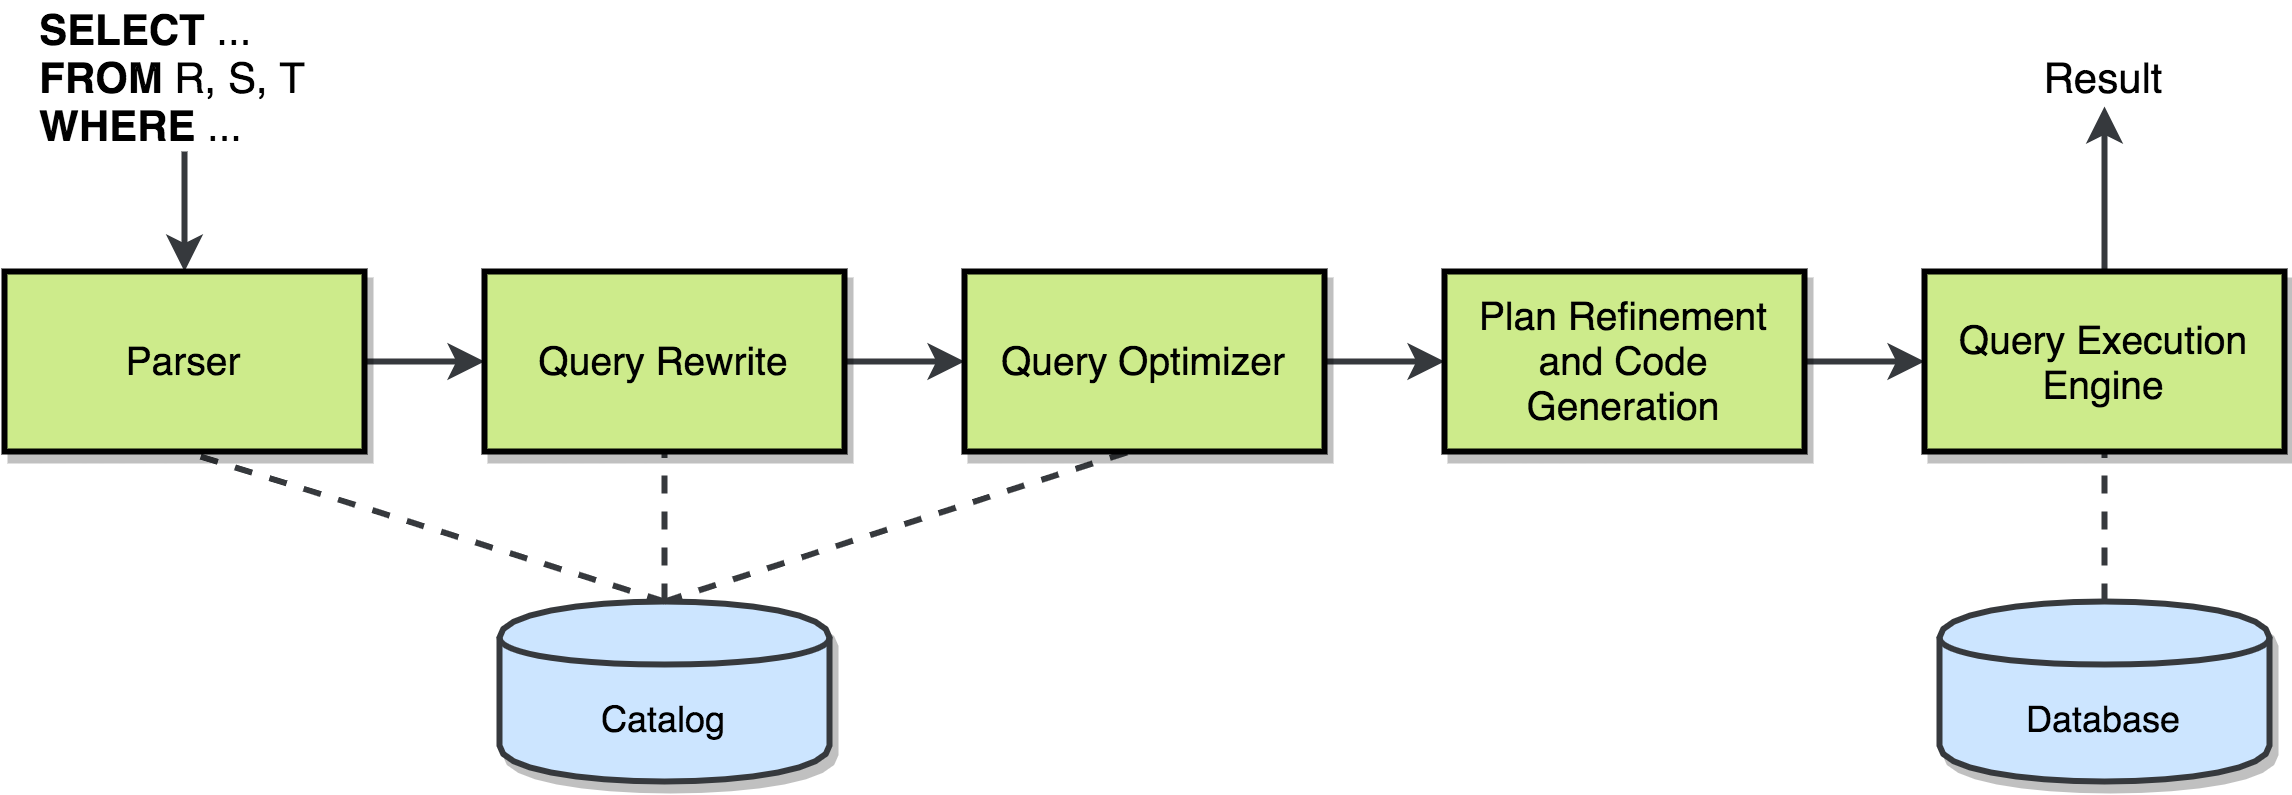
\includegraphics[width=0.95\textwidth]{img/state_of_the_art/architecture_of_a_query_processor.png}
\caption{Query processing steps \citep{Kossmann2000}}
\label{fig:query_processor}
\end{figure}

\subsubsection{Parser}

As the \gls{sql} statement itself provides an abstraction to lower-level details, it needs to be parsed and translated into an internal representation to be later optimized. This is the primary function of the parser.

\subsubsection{Query Rewrite}

In this stage, multiple transformation rules that do not depend on the system's physical state are applied. Such rules are good choices regardless of the size of the tables, the existence of index structures, locations of copies of tables, and computational power. This process includes eliminating redundant predicates, simplifying expressions, and \textit{unnesting} subqueries. % In a distributed system, the selection of table partitions must also be taken into account.

\subsubsection{Query Optimizer}

The query optimizer applies transformations that depend on the physical state of the system. For example, it determines the indices to use when executing the query, the methods (e.g., hashing or sorting) to use when executing the operations involved (e.g., joins and group-bys), and the order in which they should be executed. %Additionally, in a distributed system, the optimizer determines where each operation should be carried out. 
These decisions are made following a cost model and enumerating several alternative execution plans that return the same result.

\subsubsection{Plan}

A plan specifies how a particular query should be executed. Generally, query plans resemble traditional tree structures. Each node represents a query operator (e.g., join, group-by, sort, scan), and the edge between nodes represents the parent-child relationship between them. %In distributed systems, these can be annotated, indicating, for example, where an operator should be executed.

\begin{figure}[ht]
\centering
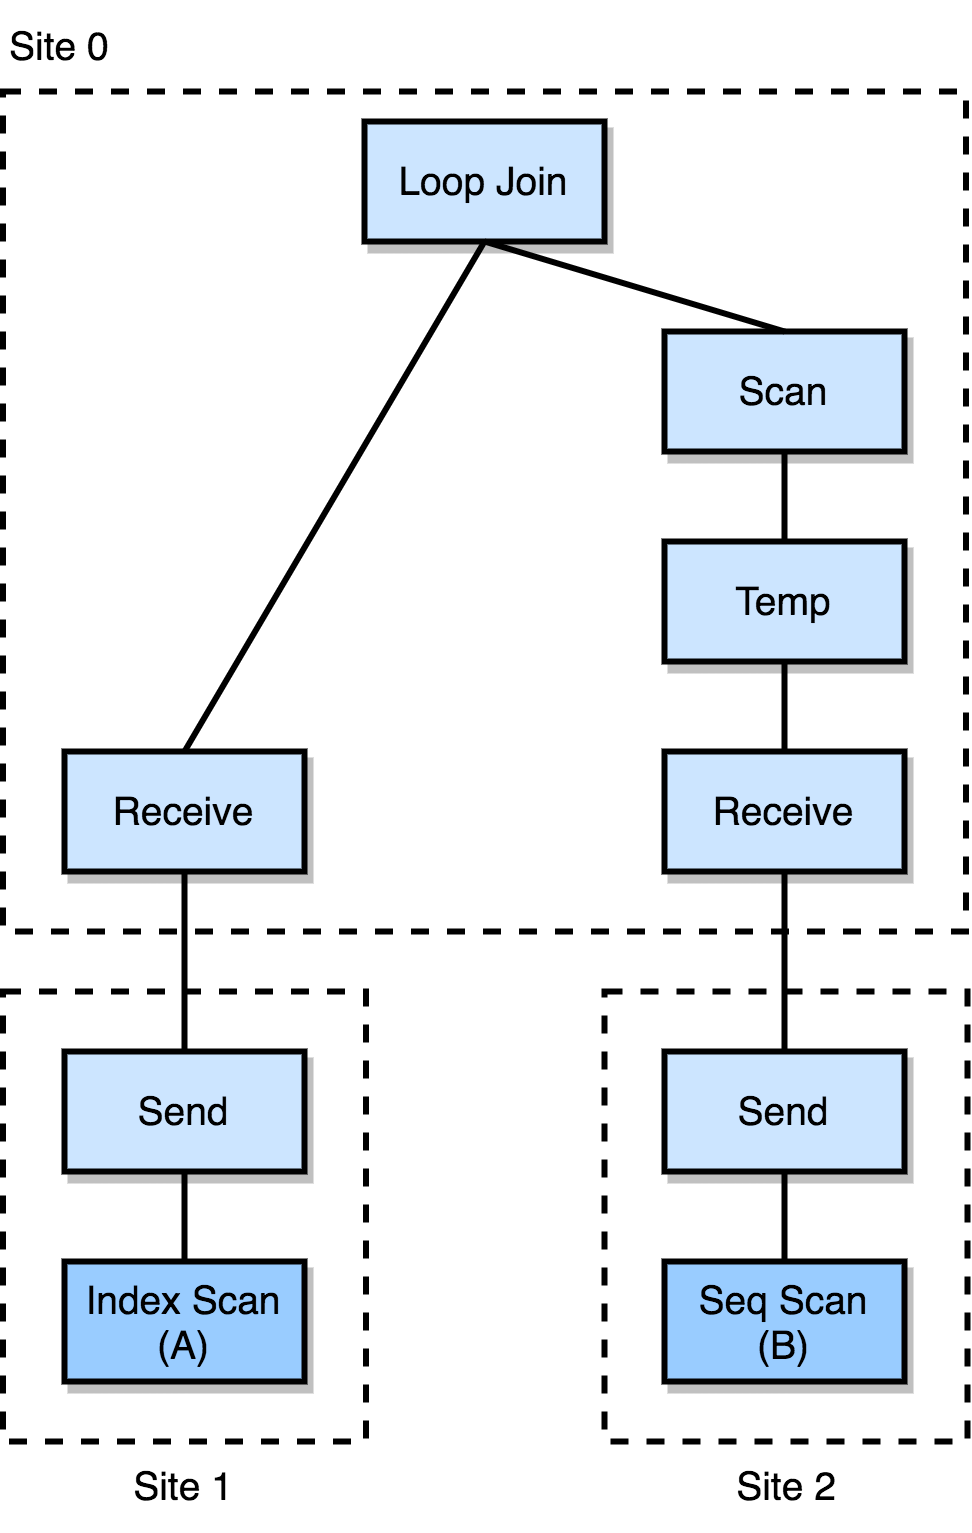
\includegraphics[width=0.4\textwidth]{img/state_of_the_art/execution_plan.png}
\caption{Example of a query execution plan \citep{Kossmann2000}}
\label{fig:execution_plan}
\end{figure}

Figure \ref{fig:execution_plan} shows an example execution plan for a query that involves two different Tables: $A$ and $B$. It specifies that \textit{Table A} is scanned at \textit{Site 1} using an index, and $B$ is scanned at \textit{Site 2}. They are then shipped to \textit{Site 0} using \textit{send} and \textit{receive} operators, and $B$ is materialized and reread at \textit{Site 0}. Both tables are then joined using a nested-loop join operator.

\subsubsection{Plan Refinement and Code Generation}

In the plan refinement and code generation stage, the plan produced by the optimizer in the previous step is transformed so that it can be further interpreted and executed by the query execution engine.

\subsubsection{Query Execution Engine}

This component ensures that generic implementations for every operator (e.g., send, scan or nested-loop join) exist. Current query execution engines are based on an iterator model \citep{Graefe1993b}, where operators are implemented as iterators that share the same interface. This allows combining two different iterators (following the consumer-producer relationship of a plan), meaning that any plan can be executed. Another advantage of the iterator model is that it supports the pipelining of results from one operator into another to improve query execution performance.

\subsubsection{Catalog}

As mentioned earlier, the optimization effectiveness depends on statistics regarding the state of the database. The catalog stores all the information needed for optimization. It maintains the database schema, partitioning schema, and physical information about the database. In traditional relational database systems, the catalog information is stored in tables. %In a distributed environment, different approaches can be considered when it comes to catalog storage. The most obvious one is to store the catalog at one central site. However, it may make sense to replicate the catalog at several sites to reduce communication costs. Nevertheless, as the catalog's size grows and is frequently updated, one strategy taken into account is to store various partitions of catalog data where it is most needed.

\bigbreak

\noindent It is important to note that, even though the architecture represented in Figure \ref{fig:query_processor} is the most widely used today, other alternatives have emerged over time. For example, many commercial database systems use architectures such as Volcano \citep{Graefe1993} and Cascades \citep{Graefe1995}, where query rewriting and optimization steps proceed as one.

Query processors may also differ in various aspects, such as the optimization granularity. For instance, there have been proposals to optimize multiple queries at a time \citep{Sellis1988}. This approach can be efficient if the queries are similar, even if the search space significantly increases.

\subsection{Basic Optimization Approach and Techniques}
\label{sec:basic_optimization_approach}

This section addresses the basic approach and strategies for optimizing queries. It first explains how a dynamic programming algorithm enumerates alternative query execution plans and then defines how different cost models can be used to estimate a particular plan's execution cost.

\subsubsection{Plan Enumeration with Dynamic Programming} 
\label{sec:dynamic_programming}

In this type of approach, the execution plan is created at compile-time and only later executed by the \gls{dbms} engine. The conventional strategy to optimize this type of queries goes back to the dynamic programming algorithm used in System R \citep{Selinger1979} and is currently implemented in most commercial systems.

\begin{figure}[ht]
\begin{algorithm}[H]
\SetAlgoLined
\DontPrintSemicolon
\KwIn{$QT$: query tree with $n$ relations}
\KwOut{$output$: best QEP (Query Execution Plan)}
\Begin{
 \For{each relation $R_i \in QT$}{
    \For{each access path $AP_{ij}$ to $R_i$}{
        compute cost($AP_{ij}$)\;
    }
  best $AP_i \longleftarrow AP_{ij}$ with minimum cost\;
  \For{each order ($R_{i1}, R_{i2},...,R_{in}$) with $i = 1,...,n!$}{
    build QEP (...((best $AP_{ij} \bowtie R_{i2}) \bowtie R_{i3}) \bowtie ... \bowtie R_{in}$)\;
    compute cost (QEP)\;
  }
  $output \longleftarrow$ QEP with minimum cost\;
 }
}
\caption{Plan Enumeration with Dynamic Programming}
\end{algorithm}
\caption{Simplified version of the dynamic programming algorithm \citep{Ozsu2011}}
\label{fig:dynamic_programming}
\end{figure}

The simplified version of the algorithm is shown in Figure \ref{fig:dynamic_programming}. It involves two loops that operate in a bottom-up fashion, building more complex plans through simpler ones. In the first step, the optimizer selects the best access method for each table referenced in the query. To do so, it exploits the predicates and access paths available for each table and estimates the cost for each alternative plan. For instance, if a hypothetical Table $A$ is replicated in sites $S_1$ and $S_2$, the algorithm would enumerate $scan (A, S_1)$ and $scan (A, S_2)$ as two possible alternatives to use in the final plan.

If the query involves more than a single table, the optimizer will explore all possible join sorting permutations ($n!$ possibilities for $n$ relations). Permutations are produced by the dynamic construction of a tree with alternative strategies. It is relevant to mention that the algorithm does not consider all possible permutations since some are not of interest. For example, permutations involving Cartesian products and the commutative equivalent strategies with the highest cost are not considered. With these two heuristics, the number of strategies examined has an upper bound of $2^n$ rather than $n!$. Inefficient plans are discarded (i.e., pruned) as soon as possible. A plan can be discarded when there is an alternative at a lower cost. For example, $A \bowtie B$ and $B \bowtie A$ would be considered two possible alternatives, but only one of them would be considered in the optimal plan. This step reduces the complexity of query optimization as it prevents more complex plans from being obtained from simpler and inefficient ones.

\subsubsection{Cost Model and Cardinality Estimation}

An optimizer's cost model predicts the cost of a given execution plan and relies on functions to predict the cost of operators, statistics and base data, and formulas to evaluate the size of intermediate results. Using cardinality estimates as its primary input, estimating the cost of a particular query execution plan typically includes estimating the cost of all operators involved and summing them up.

Cardinality estimates are usually computed based on simplifying assumptions such as uniformity and independence. The principle of uniformity assumes that all values, except for the most common ones, have the same number of tuples. On the other hand, the principle of independence assumes that predicates on attributes are independent. For joins, certain cardinality estimators follow the principle of inclusion, where the domains of the join keys overlap such that the keys from the smaller domain have matches in the larger domain.

\subsection{Dynamic Optimization Approach and Techniques}
\label{sec:dynamic_optimization_approach}

Even though the traditional approach outlined in the previous section is widely accepted, there has been a concern over the years that cost estimates lead to too many errors since many data sources do not provide reliable statistics about the system's state. Since certain assumptions made at compile-time rarely hold throughout query processing, the accuracy of the information the optimizer considers changes over time. In addition, specific parameter values may not be known until runtime. For this reason, questions about the timing of the optimization were raised, and adaptive query processing techniques were developed, allowing execution plans to be altered at execution time.

\paragraph{Dynamic Query Evaluation Plan}

\citep{Cole1994} introduced the idea of generating several alternative plans or sub-plans at compile-time, save them in the database and choose the plan that best fits the state of the system right before its execution. The approach is primarily static given that dynamic execution plans are initially produced using a dynamic programming algorithm as the one described earlier in Section \ref{sec:dynamic_programming}. However, certain optimization decisions may occur at runtime. For instance, it is possible to use choose-plan operators when two different plans are incomparable. Two or more equivalent plans are incomparable at compile time when important runtime information (e.g., parameter bindings) is missing to estimate cost.

\paragraph{Decomposition}

\citep{Ozcan1997} developed a strategy for processing queries where the general procedure consists of two steps. First, in query decomposition, the query is rewritten into a group of sub-queries, each targeted at a single data source, based on information acquired on the fly. Second, the query scheduler explores the potential parallelism and execution dependencies between the different sub-queries to restrain the search space and optimal query execution schedule. This minimizes the overall response time and, consequently, reduces the total query processing cost.

\paragraph{Continuously Adaptive Query Processing}

Eddies \citep{Avnur2000} is a query optimization system that continuously reorders operators in a query plan as it runs by merging the optimization and execution stages. This allows each tuple to have a flexible ordering of the query operators. It is possible for query plans to be reordered using two different principles: (1) synchronization barriers where inputs from different sources are coordinated and (2) moments of symmetry where pipelined joins are easily reordered.
            
    \section{Foundations of Machine Learning}
    
        Machine learning is currently a hot topic for many reasons. The most important is that it can recognize unknown patterns and make decisions based on data-driven predictive models without being explicitly programmed to do so.

There are obvious questions that need to be answered to implement machine learning systems properly. Having several algorithms to choose from, the answer to these questions varies depending on different situations as no single algorithm works for all of them. There are many factors at work, such as the size and structure of the available data, the purpose of using machine learning in that particular scenario, and the available computational power. This section provides a better understanding of the multiple paradigms, tasks, and the most common machine learning algorithms currently available.

\subsection{Learning Process Overview}

Machine learning algorithms rely on historical data (i.e., a data set) typically represented as a table, where each row represents an instance or data point. Each column represents the features of that instance and its corresponding values. 

The data set is usually split into at least two different subsets, a training data set, in which a predictive model is built from, and a test data set to determine the model's predictive accuracy. Usually, an optional third validation set may be created as well.

As mentioned earlier, machine learning algorithms use statistics and mathematical optimization to automatically find unknown data patterns and predict some target output or response. The optimization process generally involves finding the minimum or maximum value of a function, often referred to as a loss or cost function.

\subsection{Types of Learning Algorithms}

Different machine learning algorithms differ in their approach, the type of data used as input and output, and the type of task or problem they are intended to solve. This subsection discusses the different types of algorithms available.

\subsubsection{Supervised Learning}

In supervised learning, the input data has a known label or result. The goal is to predict a target variable of the unseen data given a set of variables or features. The algorithms build a predictive model on labeled historical data and learn relationships between the input and label variables. Table \ref{tab:supervised_learning} shows a typical simple example of a supervised learning problem, where the target variable to be predicted is the class of the iris plant.

\begin{table}[H]
\begin{tabular*}{\textwidth}{p{0.17\textwidth} p{0.17\textwidth} p{0.17\textwidth} p{0.17\textwidth} p{0.20\textwidth}}
\hline
\multicolumn{4}{c}{\textbf{Features}}                                                                                                               & \textbf{Target Variable}  \\ \hline
\textit{\textbf{Sepal Length}} & \textit{\textbf{Sepal Width}} & \textit{\textbf{Petal Length}} & \textit{\textbf{Petal Width}} & \textit{\textbf{Species}} \\ \hline
5.1                                 & 3.5                                & 1.4                                 & 0.2                                & setosa                    \\
4.9                                 & 3.0                                & 1.4                                 & 0.2                                & setosa                    \\
4.7                                 & 3.2                                & 1.3                                 & 0.2                                & setosa                    \\
4.6                                 & 3.1                                & 1.5                                 & 0.2                                & setosa                    \\
5.0                                 & 3.6                                & 1.4                                 & 0.2                                & setosa                    \\ \hline
\end{tabular*}
\caption{Example of supervised learning naming conventions}
\label{tab:supervised_learning}
\end{table}

A predictive model's quality is measured using an independent test set to evaluate whether the discovered relationships are helpful in unseen scenarios. By feeding the model with input variables of the test data, it is possible to compare its predicted label with the data's actual label. The evaluation process typically involves a proportional split between train and test data. A more significant proportion of test data ensures a better performance validation. In contrast, insufficient training data means that the model has fewer data to learn from.

\subsubsection{Unsupervised Learning}

Unsupervised learning involves learning from data with no label or response variable and is more about finding patterns than prediction. It is referred to as unsupervised since it lacks a response variable that can supervise the analysis. Considering that no labels are available for input data, a model is built by deducting hidden input data patterns.

\subsubsection{Reinforcement Learning}

The reinforcement learning approach is illustrated in Figure \ref{fig:reinforcement_learning}. The algorithm interacts with an environment and learns to optimize its behavior over a continuous feedback system of rewards and punishments to maximize the numerical value of reward over a given amount of time.

\begin{figure}[H]
\centering
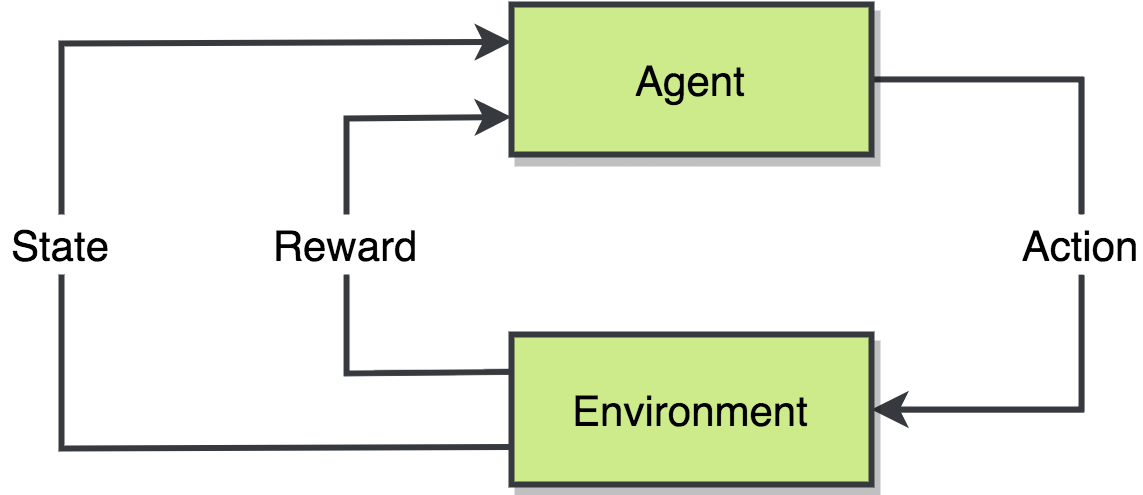
\includegraphics[width=0.6\textwidth]{img/state_of_the_art/reinforcement_learning.png}
\caption{Reinforcement learning}
\label{fig:reinforcement_learning}
\end{figure}

In contrast to supervised learning, the agent observes the current state and decides what to do, predicting the expecting future, so the agent is bound to learn from its experience. Reinforcement learning focuses on online planning and requires a balance between exploration (of the unknown) and exploitation (of existing knowledge).

\subsection{Tasks}
\label{sec:machine_learning_tasks}

A machine learning task refers to the type of prediction or inference being made based on the problem or question being asked and the available data. This subsection describes the different machine learning tasks and some of their conventional use cases.

\subsubsection{Classification}

Classification is a supervised machine learning task in which one or more classes are assigned to each instance based on a set of values for the input variables. It has different types depending on the number of output classes available: binary classification when there are two classes and multi-class classification when there are three or more classes. It is important to note that it differs from multi-label classification, where an instance can be assigned to multiple labels.

\subsubsection{Regression}

Target variables can be either numerical or categorical. While classification problems are associated with categorical labels, regression tasks refer to problems with a numerical target variable. Regression algorithms model how the variation in the values of features translates into a numerical label.

\bigbreak

\noindent Even though classification and regression are the most popular tasks, there are other types of tasks worth mentioning:

\begin{itemize}
    \item \textbf{Clustering} where the main goal is to group instances of data into clusters that contain similar characteristics by identifying relationships in a data set that one can not merely derive by browsing or simple observation;
    \item \textbf{Anomaly Detection} that identifies rare events or observations that differ significantly from the majority of the data;
    \item \textbf{Recommendation Systems} that can produce a list of recommended products or services to a given user. These systems can use a single input or multiple inputs within and across platforms, such as items, users, and transactions.
\end{itemize}

\subsection{Algorithms}
\label{sec:machine_learning_algorithms}
There are many algorithms proposed in the literature, each with its advantages and limitations depending on the task at hand and the data available. Commonly used machine learning algorithms include:

\subsubsection{Linear \& Logistic Regression}

Regression algorithms infer the relationship between output labels and the corresponding input data features. The main difference between linear and logistic regression relies on the type of dependent variable. In linear regression, it is continuous, while in logistic regression, it is discrete.

\subsubsection{Decision Trees}

Decision trees are used for both regression and classification problems based on the data's actual attributes. Each node represents a feature of a given instance, and each branch represents a decision. The leaves represent an outcome, which can be either categorical or numerical.

\subsubsection{Association Rules}

Association rule learning algorithms are a form of rule-based machine learning method to discover associations between data variables. Each rule is formed of an antecedent and a consequent, enabling the discovery of frequent patterns or association structures within a data set.

\subsubsection{Support Vector Machines}

Support Vector Machine can be used for both classification and regression problems and divides the data samples of two classes by determining a hyper-plane in input space that maximizes the separation between them and classifies new cases to one of the two groups.

\subsubsection{Genetic Algorithms}

Genetic Algorithms view learning in terms of competition among a population of evolving, alternative concepts. A genetic algorithm maintains a population of candidate problem solutions. According to their performance, only the fittest of these solutions survive and exchange information with other candidates to form new solutions.

\subsubsection{Artificial Neural Networks}

Artificial Neural Networks, inspired by biological neural networks, comprise basic processing units called neurons, connections, and weights. During the learning process, the weights of the connections are updated over time using a backpropagation algorithm to model the dependencies between input features and target variables.

Deep learning refers to a large and deep artificial neural network with many more layers and many more nodes in each layer, resulting in many more parameters to tune.
The higher amount of available data and computational power are the reason for its sudden popularity over the years.

\paragraph{Convolutional Neural Networks}

A convolutional neural network (\gls{cnn}) is a particular type of neural network that takes an image as input. It can differentiate one image from the other by assigning importance through learnable weights and biases to various traits or objects in the image. As illustrated in Figure \ref{fig:convolutional_neural_networks}, it has convolutional layers that intend to capture the high-level features from the input image, and pooling layers, responsible for reducing images into an acceptable size that is easier to process without losing the convolved feature, which is a critical step for getting the right prediction.

\begin{figure}[H]
\centering
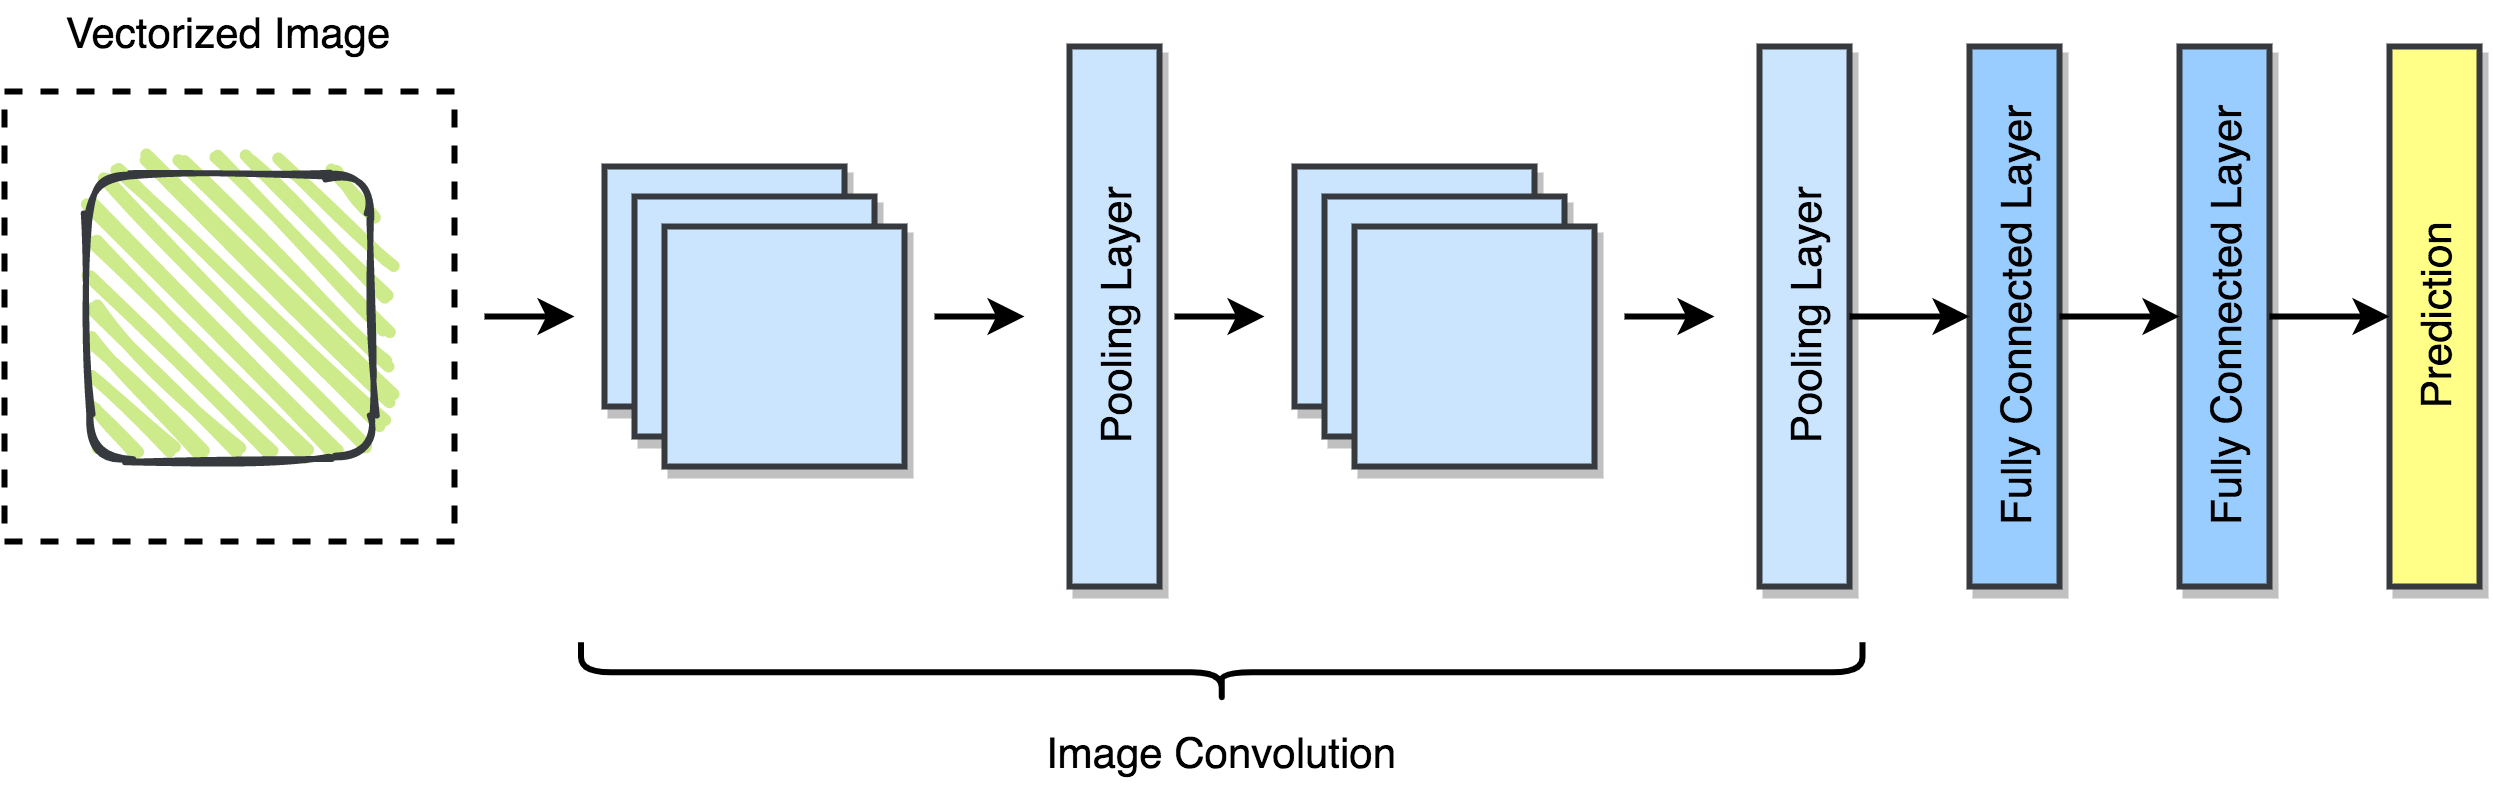
\includegraphics[width=\textwidth]{img/state_of_the_art/convolutional_neural_network.png}
\caption{Convolutional neural networks}
\label{fig:convolutional_neural_networks}
\end{figure}

The actual learning process is done by feeding the flattened output of the high-level features (i.e., the convolutional layer's output) to a feed-forward neural network and applying the backpropagation algorithm to every training iteration. Thus, over a series of epochs, the model can distinguish between dominating and certain low-level features in images.
        
    \section{Machine Learning in Query Processing}
    
        Section \ref{sec:foundations_of_query_processing} has shown that despite the progress made over the past decades, query optimizers continue to be highly complex components with well known limitations. The challenge of enumerating a set of candidate execution plans and identifying the most efficient has a prominent trade-off. Searching a larger search space increases the likelihood of finding the optimal plan but requires spending more time on query optimization than desired.

As described earlier, current database systems use a set of heuristics to limit the search space at the cost of missing potential good plans to reduce the search space and optimization time as a result. More importantly, they use static strategies that do not learn from past experiences risking selecting the same bad plan multiple times and, therefore, never learning for its bad choices.

Data-driven machine-learning-based applications success has left the database research community wondering whether it was possible to integrate machine learning techniques in query processing and optimization. Having described both the foundations of query processing and machine learning, this section explores how the two can overlap and looks into more detail on the many attempts made over the last few years to apply machine learning to modern query optimizers. The majority of this work has focused on replacing a single component of the optimizer with learned models.

\subsection{Join Ordering}

As the join order's permutations have a critical effect on the performance of relational queries \citep{Ozsu2011}, applying machine learning techniques to guide the search space in a more data-driven way has received a lot of attention.

ReJOIN \citep{Marcus2018a} uses a traditional cost-based approach to query optimization where an algorithm selects the most efficient ordering for execution following a cost model. The main difference is addressing the incapability of optimizers learning from past experiences by using reinforcement learning combined with the traditional cost model to automatically learn search strategies and explore the space of possible join orderings.

\subsection{Cost Model and Cardinality Estimation}

Another limitation of current query optimizers is using cardinality estimates as the optimizer's cost model principal input. There is a trade-off between the accuracy of the statistics in which they are based and their maintenance costs since more accurate statistics are significantly harder to maintain. For this reason, they are usually computed based on simplifying assumptions that are frequently wrong in real-world scenarios, which may result in poor performance \citep{Leis2015}.

In accordance with this observation, there is a proposal \citep{Kipf2018} to model the cardinality estimation as a supervised learning problem, with the input being query features and the output being the estimated cardinality. The model can further be used as an estimator for other, unseen queries.

\subsection{Performance Tuning}

Since the architecture of query optimizers have the inherent limitations mentioned above, database knob tuning became an incredibly important task to provide a higher level of flexibility to meet specific requirements and achieve higher performance. The problem is that databases have hundreds of knobs which are typically pragmatically adjusted by \gls{dbas} based on response time analysis~\citep{ferreira2020self,vanaken17}.

Bao \citep{Marcus2020} is a learned system that is capable of learning what execution strategy the query optimizer should use by limiting the search space of the traditional optimizer on a per-query basis. It is a reinforcement learning-based approach that observes a reward value following the selection of a optimization strategy configuration.
        
    \section{Discussion}
    
        In short, many of these solutions lead to phenomenal results, confirming the potential of integrating machine learning techniques in query optimizer components. However, one could argue that, similarly to the problems they are trying to solve, they suffer from several fundamental limitations as well. Most proposed solutions are based on reinforcement learning techniques that need a substantial amount of time and queries to learn from before matching or outperforming modern query optimizers. Another problem is that they try to replace or discard state-of-the-art query optimizers entirely and do not take advantage of their readily available mechanisms. Finally, they introduce even more complexity to a system that is already complex by itself, making it even harder to understand and extend the learned component's query planning capability.

Based on the analysis of previous work, a complete and adequate solution should use the following guiding principles:

\begin{itemize}
    \item Require a short training time and amount of data to learn from. A realistic solution should not take days to train nor should it require an impractical amount of data before having a positive impact on query performance;

    \item Learn from the optimizer. Since query optimizers contain decades of meticulously research and development, the solution should leverage the valuable information obtained from their generated query plans;
    
    \item Have a high level of interpretability. It should provide a way of understanding the decisions that are made under the hood and be adjustable when leading to poor decisions while the underlying optimizer is functioning correctly;

    \item Be extensible. A good proposal should be easily extensible, making it possible to add new query plan representation techniques, machine learning algorithms and be used across different database systems.
\end{itemize}
        
\chapter{Odin}

    This chapter describes the developed solution, beginning with some experimental observations on which it is based upon, followed by a high-level architecture overview and the prototype implementation in detail.

    \section{Preliminary Experiments}
    
        \label{sec:preliminary_experiments}

As discussed in the previous chapter, the optimizer’s behavior is driven by indices, cost settings, strategy settings, and its general perception of the data distribution. Database systems come with basic configurations tuned for broad compatibility rather than optimal performance. As the default parameters may be unsuitable in some scenarios, database systems allow disabling different strategy settings on a per-query or permanent basis to dissuade the optimizer from going down an unproductive path.

To analyze the impact of enabling or disabling strategy settings on query runtime, we set up a scenario that considers an out-of-the-box PostgreSQL~\citep{PostGreSQL} server instance and two different queries from the Join Order Benchmark (\gls{job})~\citep{JOB} workload, which is described in further detaile in Section \ref{sec:workloads}. First, each query is executed without any strategy restrictions, in which all settings are enabled, and then executed with strategies that tend to be costly disabled, establishing a comparison among these settings in the end.

\begin{figure}[H]
  \begin{subfigure}[t]{0.5\textwidth}
    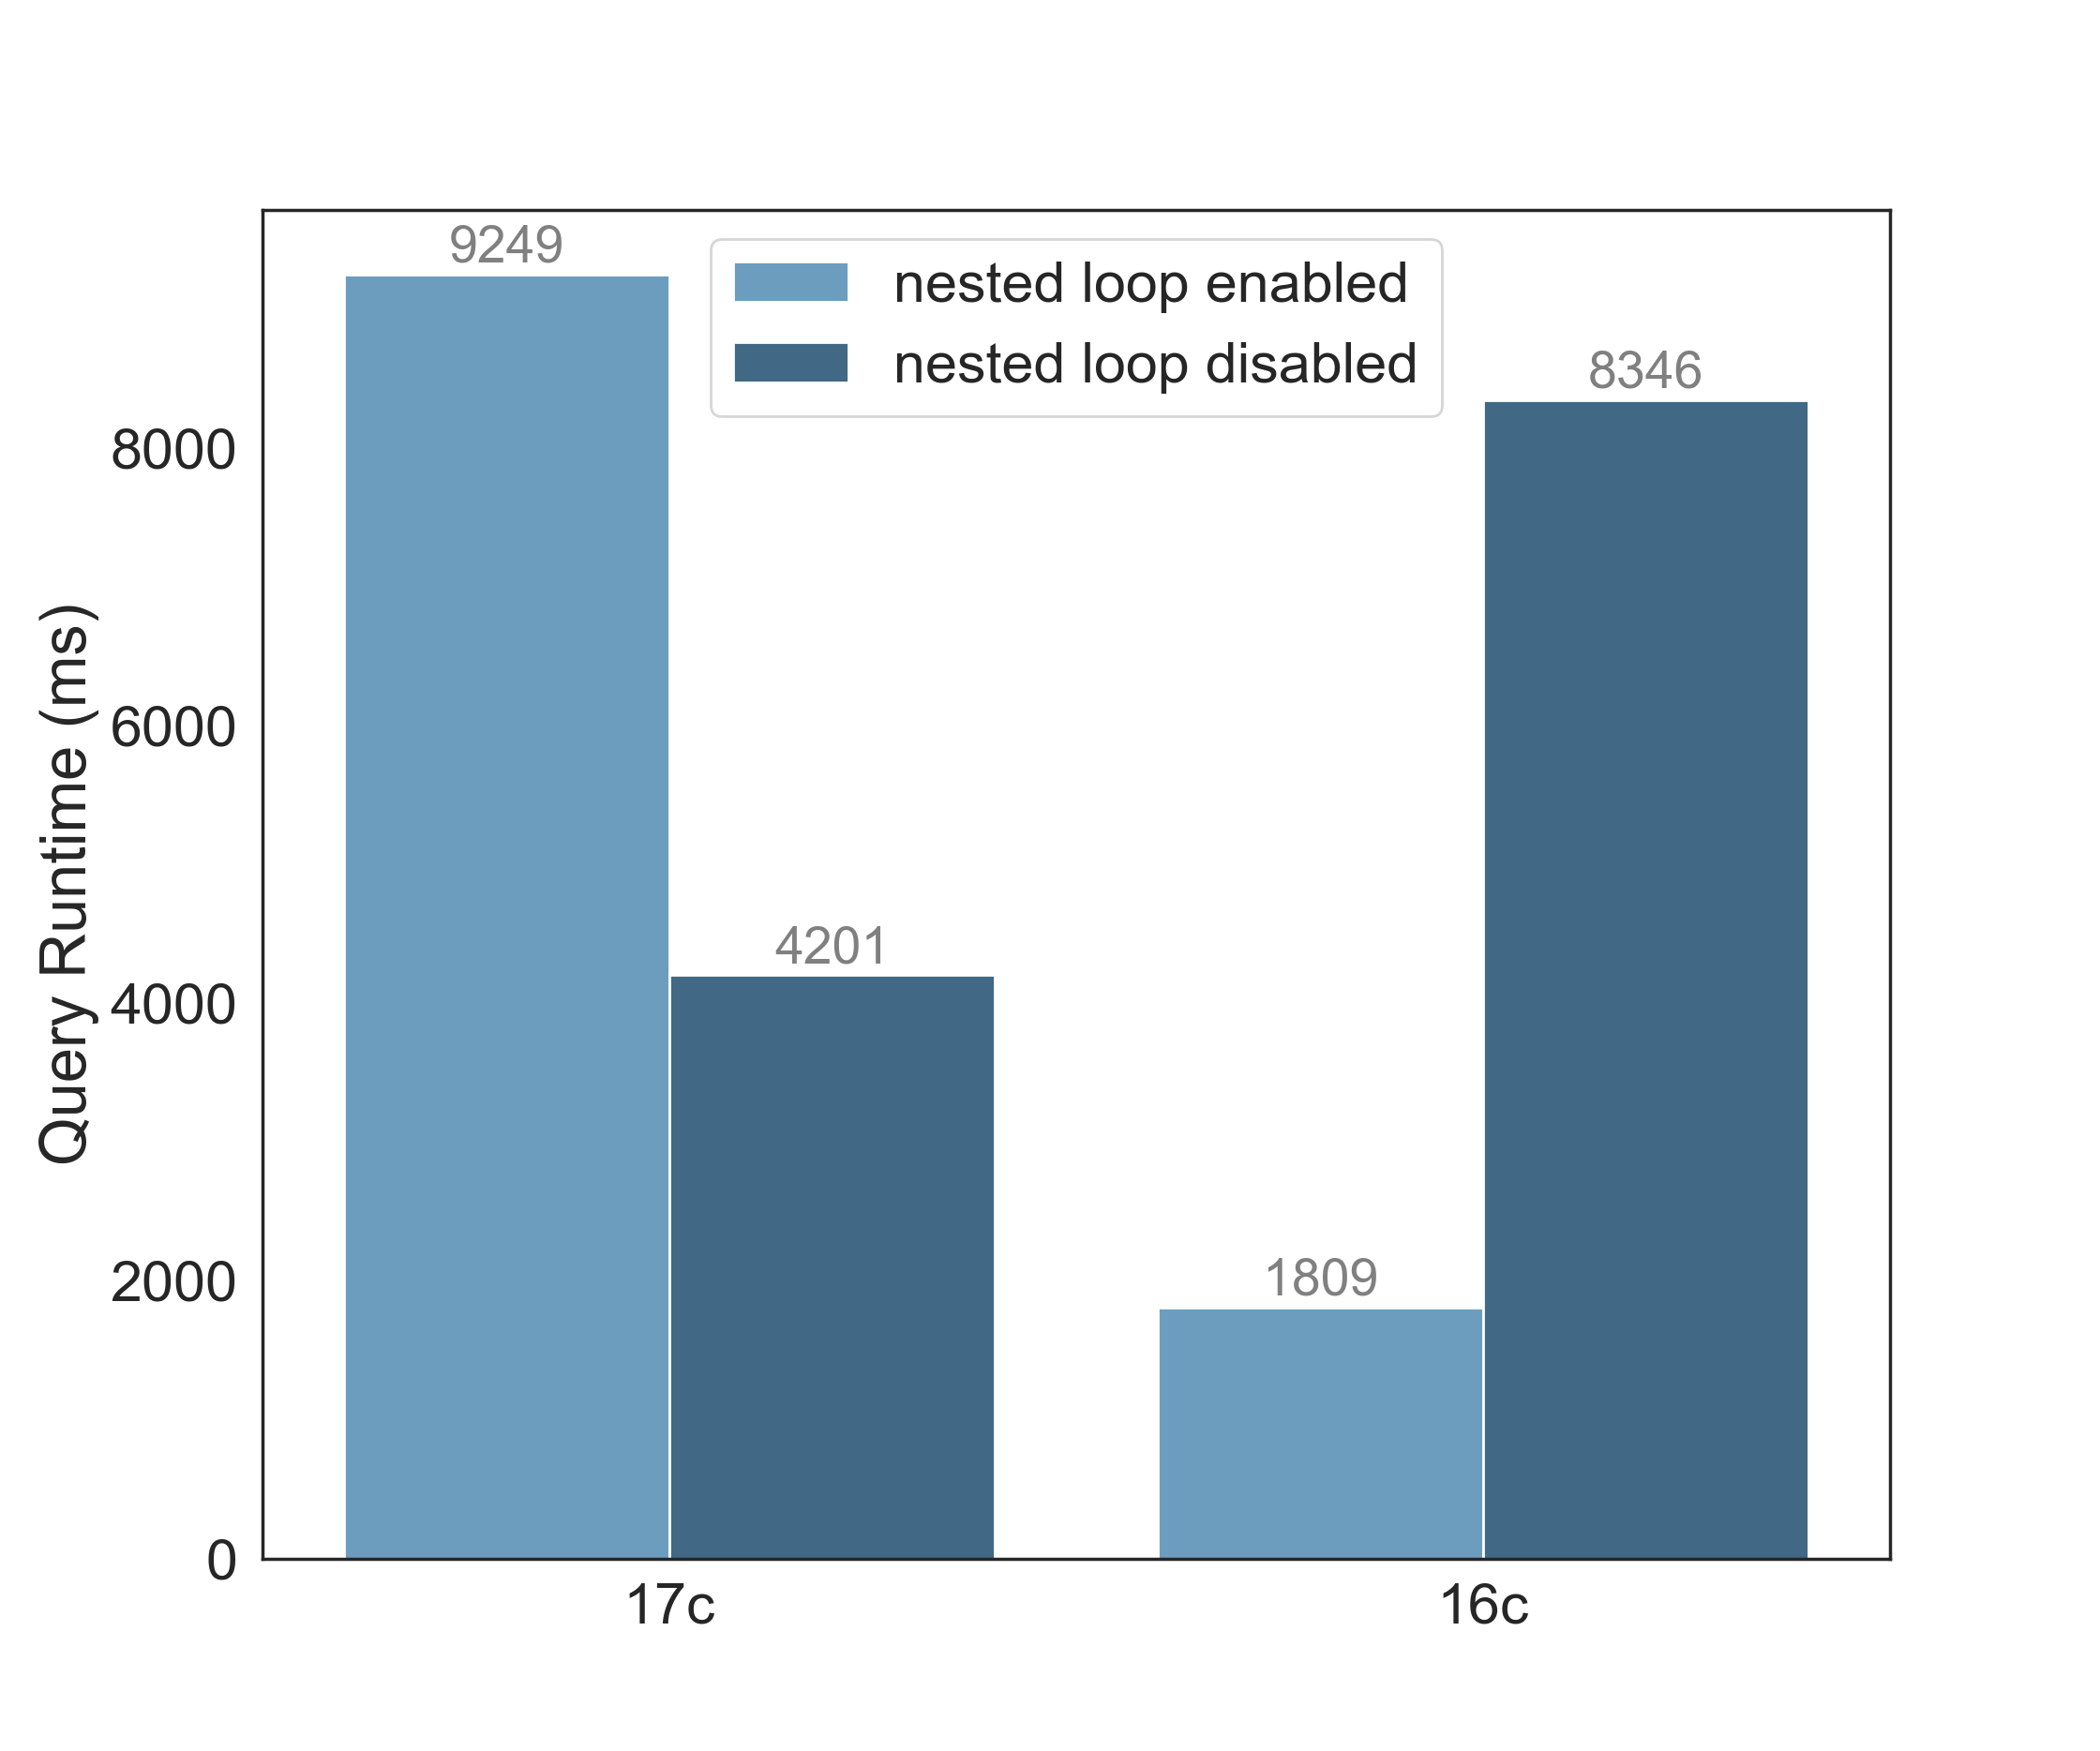
\includegraphics[width=\textwidth]{img/solution/nested_loop_experiment.png}
    \label{fig-a}
  \end{subfigure}\hfill
  \begin{subfigure}[t]{0.5\textwidth}
    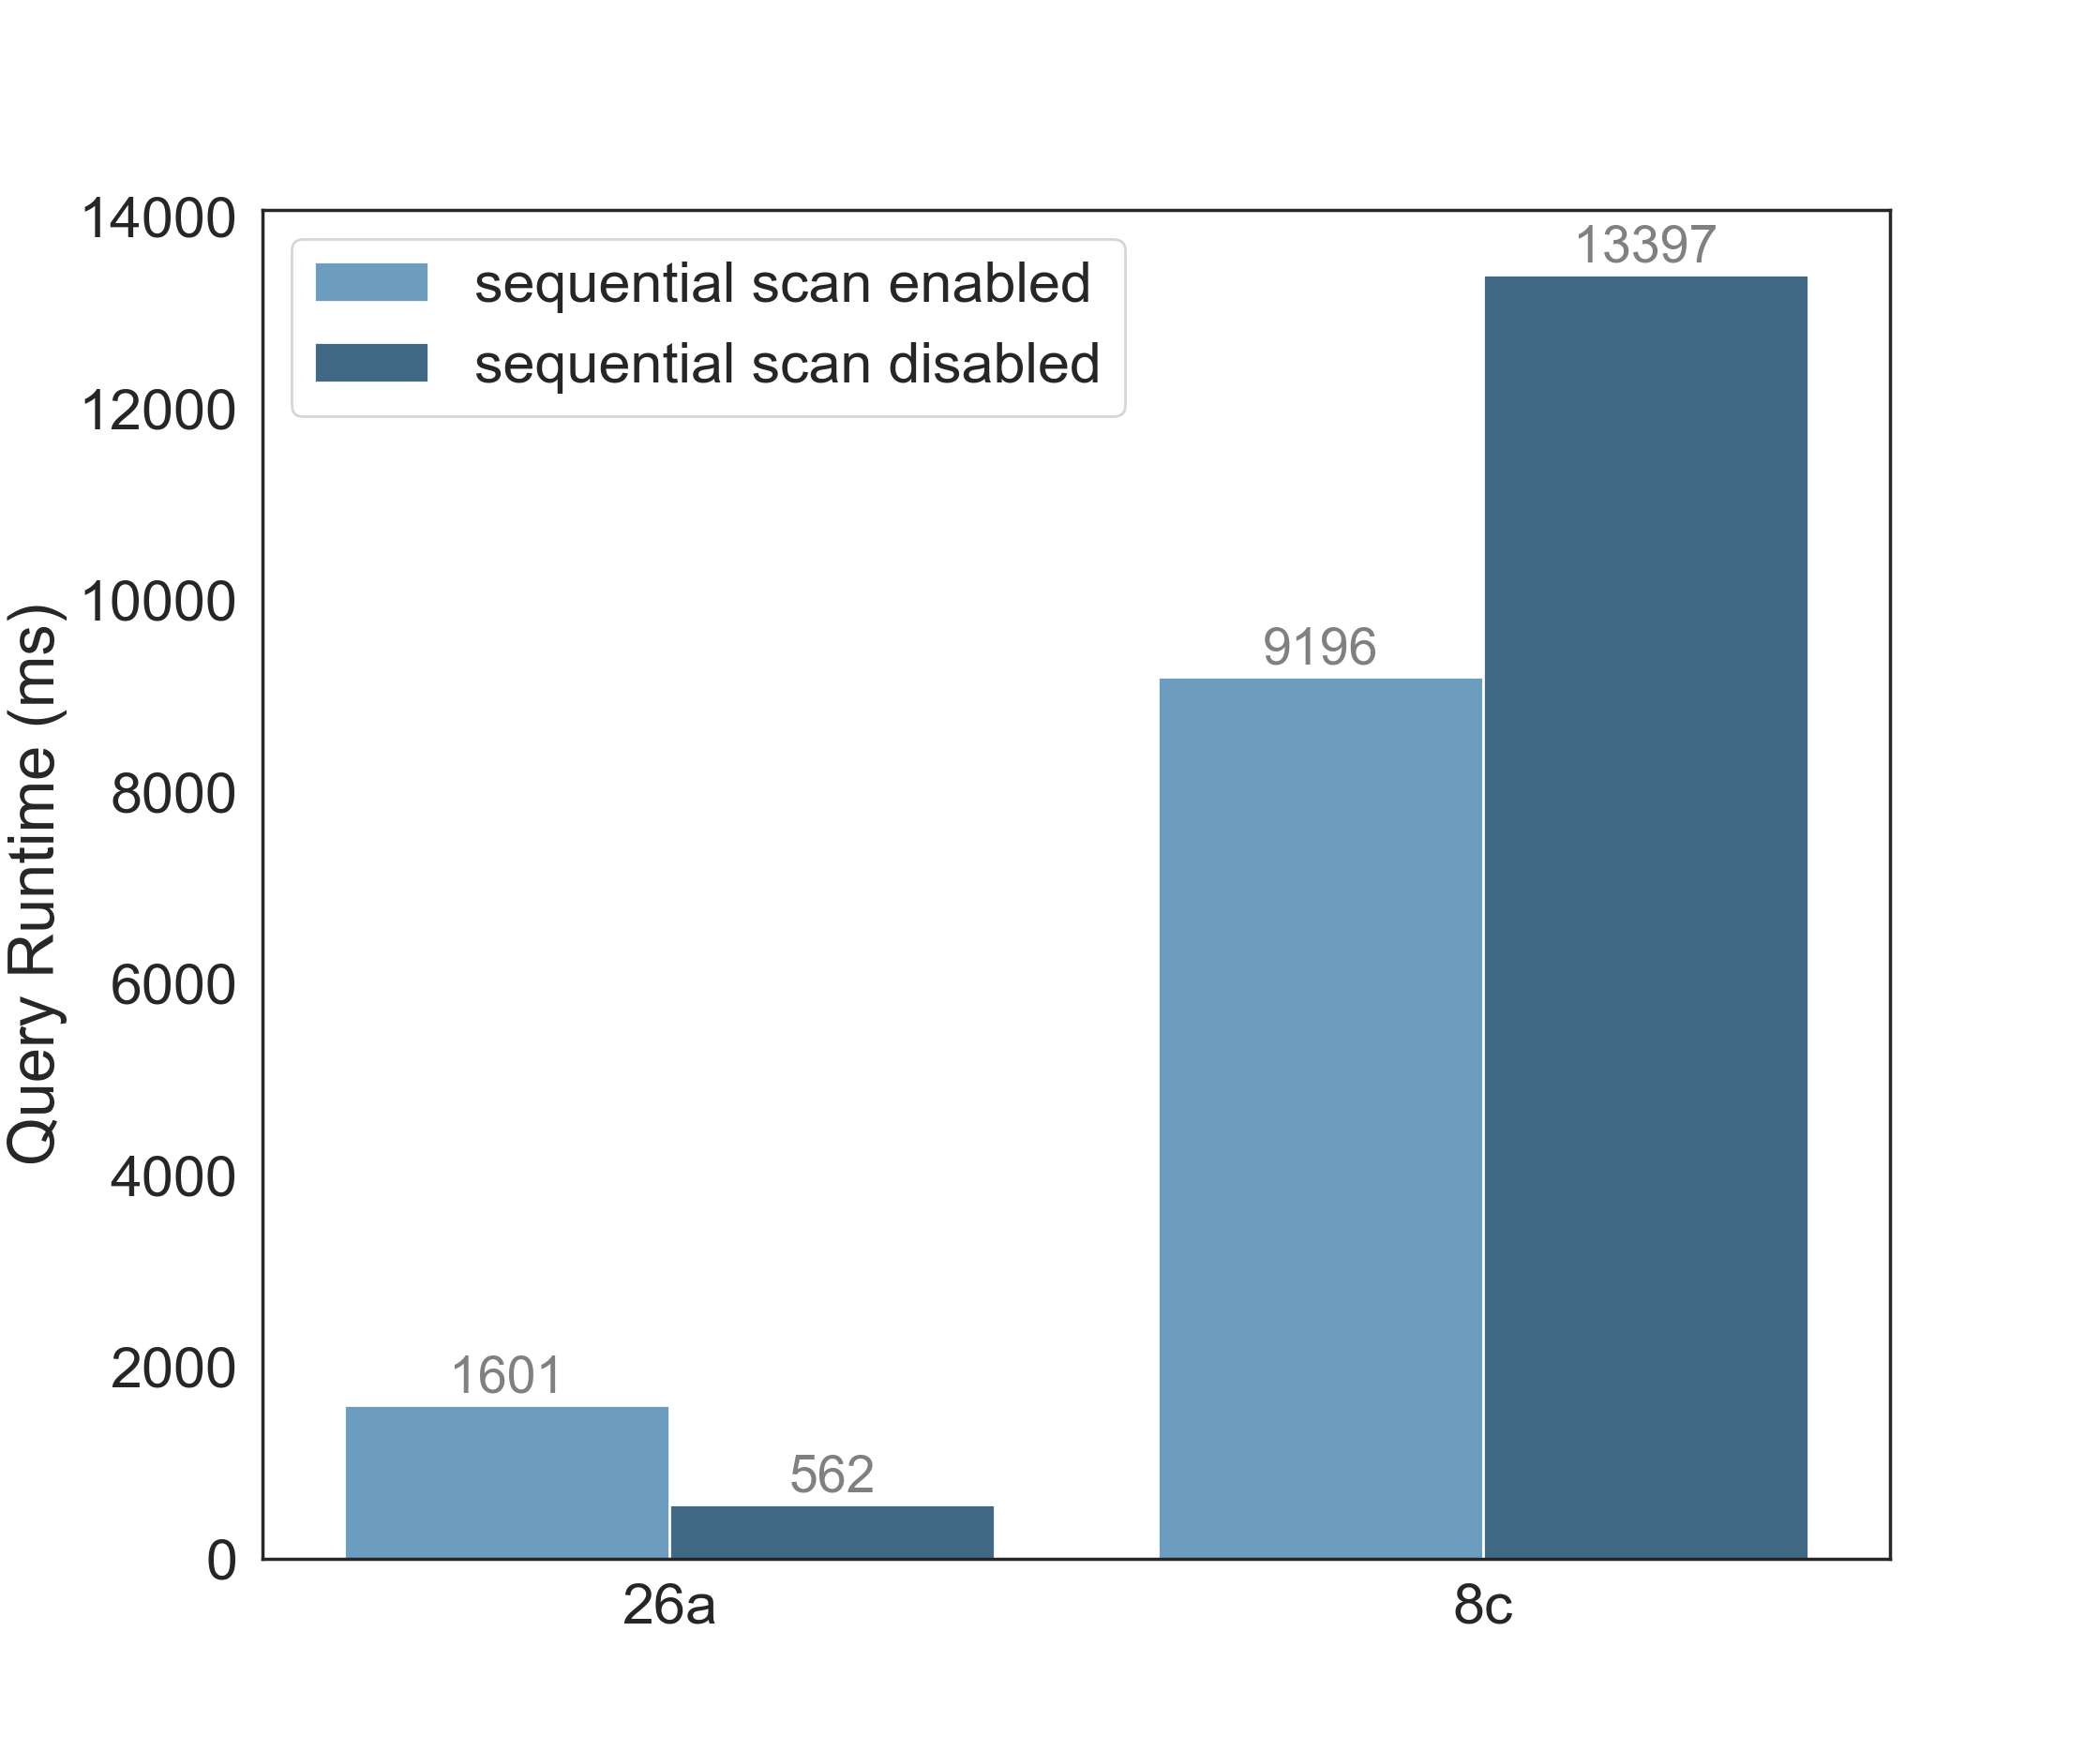
\includegraphics[width=\textwidth]{img/solution/sequential_scan_experiment.png}
    \label{fig-b}
  \end{subfigure}
  \caption{Impact of disabling strategy settings in PostgreSQL on query's performance} 
  \label{fig:preliminary_experiments}
\end{figure}

As Figure \ref{fig:preliminary_experiments} clearly illustrates, dissuading the optimizer from using strategies such as nested loop joins and sequential scans may result in substantial reductions in query execution time, despite not always being the case.

Based on this observation, one could argue that finding the best configuration for a query can significantly improve execution runtime. Having some prior knowledge of the data, database administrators can infer which operators will lead to sub-optimal performance and restrict the search space by disabling those strategies. However, most of the time, knobs are pragmatically adjusted based on response time analysis, as permanently disabling specific strategies could lead to performance degradation. For instance, for \gls{job}'s query 16b, disabling nested loop joins causes a regression in query performance.

Our solution sits on top of a conventional optimizer and learns when to enable or disable some of its strategies on a per-query basis. Effectively, the core idea is to learn the execution strategy the query optimizer should use for a particular query and maximize query performance improvements while avoiding significant regressions.

    \section{Architecture}
    
        Odin lies between the user and the relational database it is built upon, introducing learning capabilities to its query optimizer. It extends the client interface provided by the database system with commands that infer the best set of strategy settings on a per-query basis.

Upon receiving a query, it evaluates different plans under different optimizer strategy settings and tries finding the configuration that results in the lowest runtime. To do so, it relies on the underlying optimizer to produce different execution plans under different configurations. It takes advantage of query plan execution information and statistics that databases systems provide (i.e., type of operators involved, the cardinality estimates, and execution cost) before execution. These are then used to construct a vectorized representation of each plan, which is later fed into a predictive model and evaluated based on its predicted outcome.

The architecture of Odin is based on three different modules: (1) the Parser and Featurizer, (2) the Learning Module, and (3) the Configuration Tuner. Figure \ref{fig:architecture} illustrates the solution's architecture and how the different modules interact with each other. Next, we describe in further detail the role of each module.

\begin{figure}[H]
\centering
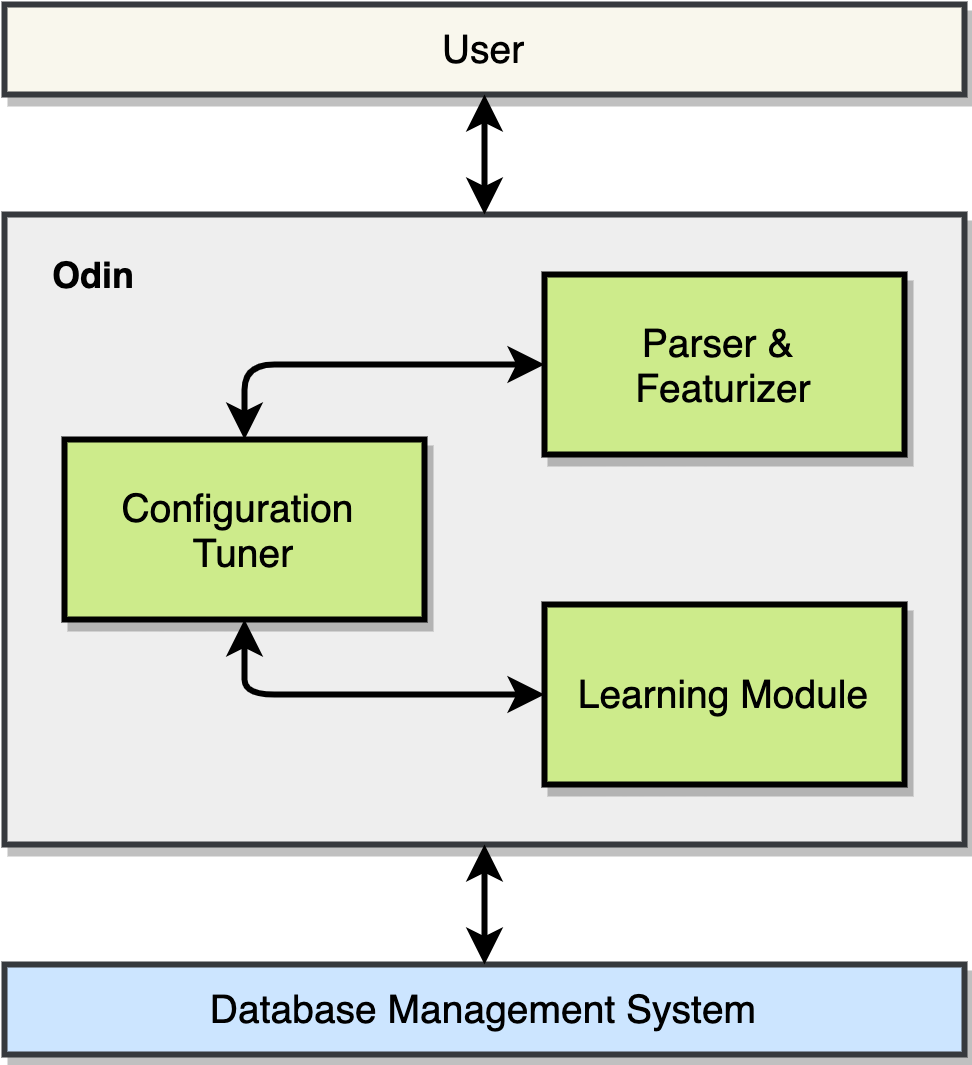
\includegraphics[width=0.5\textwidth]{img/solution/architecture.png}
\caption{Odin's architecture}
\label{fig:architecture}
\end{figure}

The \textbf{Parser and Featurizer} module contains several mechanisms for reading files that contain \gls{sql} statements and extract vector representations of query plans generated by the optimizer to be further interpreted by predictive modeling techniques.

The \textbf{Learning Module} is responsible for generating, loading, and saving several types of predictive models. The module assumes the existence of previously executed queries from which the models can be obtained and relies on the plan vector representations mentioned above and their observed runtimes.

The \textbf{Configuration Tuner} is in charge of orchestrating the communication between the two as well as enabling the selection of the best alternative optimizer configuration for a particular query. It interacts with the PostgreSQL client interface to enable or disable a set of strategies based on a direct comparison between different configurations and their expected runtime, as predicted by one of the previously trained learned models.

    
    \section{Prototype Implementation}
    
        The Odin middleware is designed to be adaptable and extensible, adopting procedures that are readily available in most relational database systems. The current prototype is built on top of PostgreSQL to enhance its optimization capabilities without replacing or discarding its optimizer completely. This section goes through the actual implementation details of each module.

\subsection{Parser and Featurizer}

This module has the task of parsing \gls{sql} statements and generate a vector representation of each alternative execution plan.

\subsubsection{Parser}

The parser reads \gls{sql} statements and interacts with the underlying \gls{dbms} interface to get an idea of how the optimizer intends to execute the query without actually running it. Most database systems come with a built-in explainer that tells how the query planner will execute a particular SQL query (e.g., \textit{EXPLAIN} command in the case of PostgreSQL). As shown in Figure \ref{fig:explain_command}, it allows targeting query performance specifics such as: (1) how the tables referenced by the statement will be scanned, (2) if multiple tables are referenced, information about what join algorithms will be used to bring together the required rows from each input table and (3) cardinality estimates and predicted execution time.

\begin{figure}[H]
\centering
\begin{minipage}{0.72\textwidth}
\begin{minted}[frame=lines,
               framesep=2mm,
               fontsize=\small,
               mathescape=true,
               escapeinside=||
]{Text}
EXPLAIN SELECT * FROM foo;

                       QUERY PLAN
---------------------------------------------------------
 Seq Scan on foo  (cost=0.00..155.00 rows=10000 width=4)
(1 row)
\end{minted}
\end{minipage}
\caption{Example of the output of an \textit{EXPLAIN} command output}
\label{fig:explain_command}
\end{figure}

\subsubsection{Featurizer}

The featurizer takes the execution plan that the PostgreSQL planner generates for the supplied statement and converts it to a vector of fixed dimensions for machine learning algorithms to interpret it. It provides a simple interface of two methods representing execution plans at two different granularities to support two different types of machine learning algorithms.

\paragraph{Plan-level Featurization}

In this method, the query plan is represented as a single vector and ignores lower-level details, such as the position and order between different operators. Instead, as illustrated in Figure \ref{fig:plan_level_featurization}, it uses a set of features containing estimates, such as operator cardinalities and execution times, together with the occurrence count of each operator type in the query plan.

\begin{figure}[H]
\centering
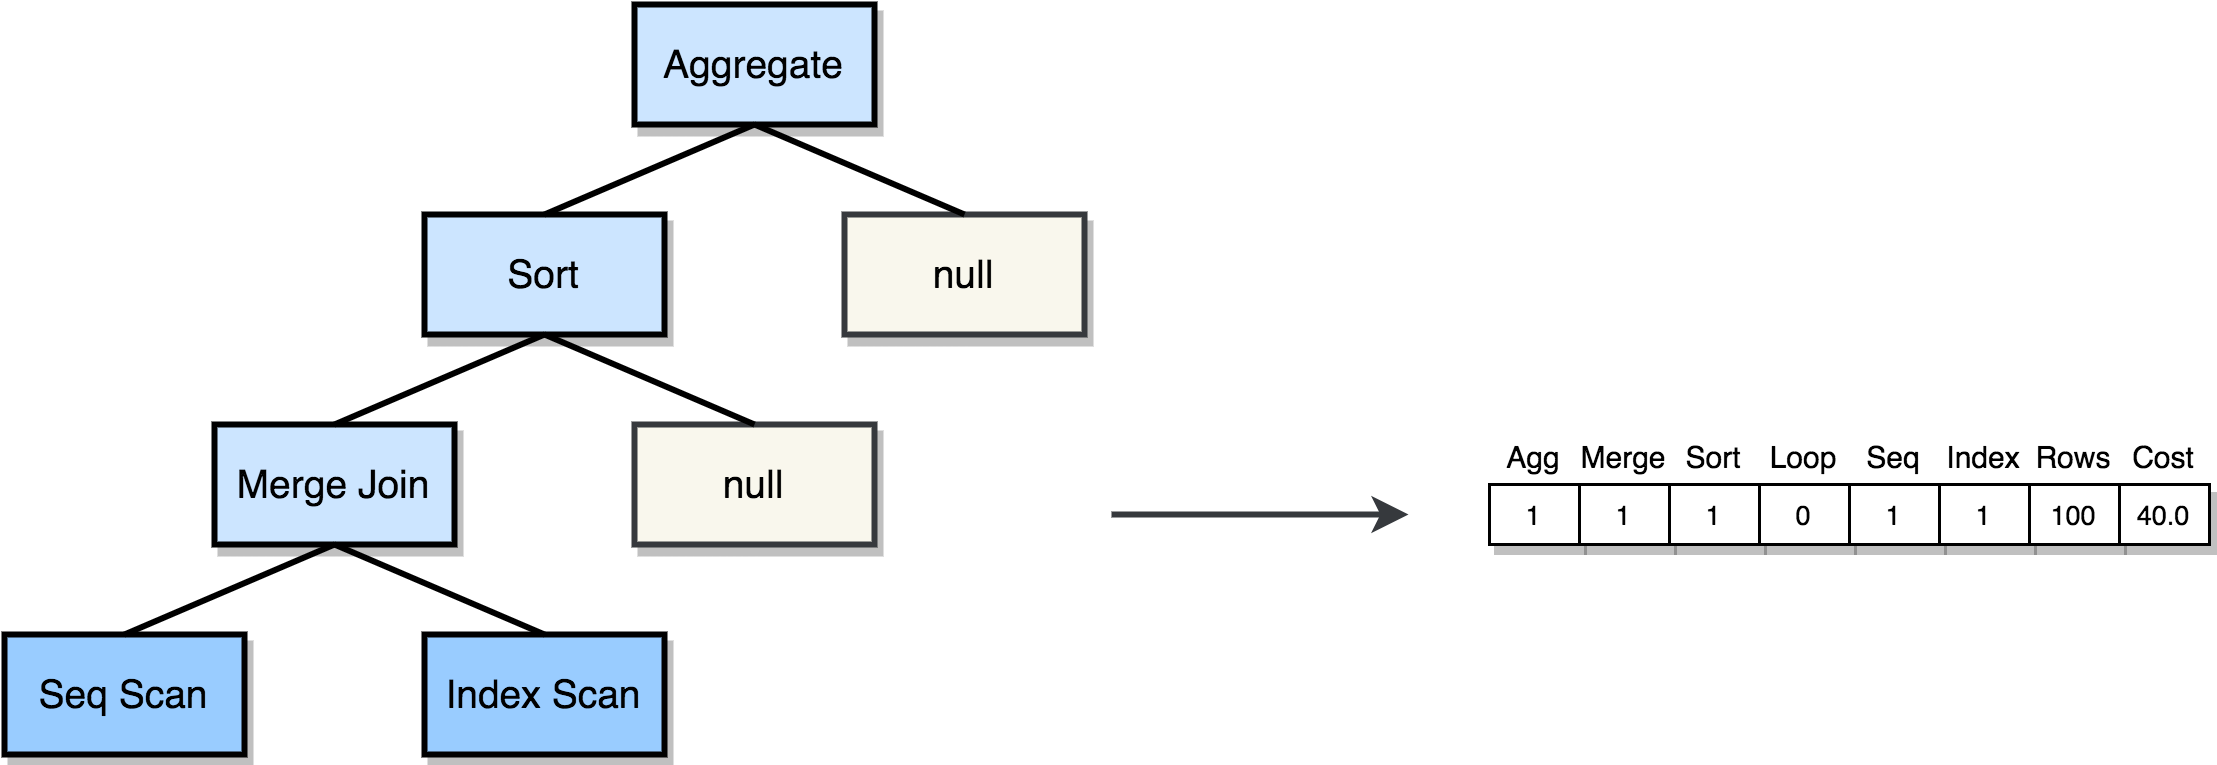
\includegraphics[width=0.9\textwidth]{img/solution/plan_level_featurization.png}
\caption{Plan-level featurization}
\label{fig:plan_level_featurization}
\end{figure}

This approach was devised to be used directly in more traditional machine learning approaches. Additionally, it is model agnostic and can readily work with different model types.

\paragraph{Operator-level Featurization}

This method encodes a query plan as a tree of vectors and preserves its inherent tree structure by binarizing the query plan tree and encoding each operator as a vector. As shown in Figure \ref{fig:operator_level_featurization}, each node is annotated by the physical operator being used and some optimizer estimates, such as estimated operator cost and cardinality. The process of binarization includes transforming non-binary query plans into binary ones by introducing \textit{null} nodes. Therefore, each tree node has exactly two or zero children. 

\begin{figure}[H]
\centering
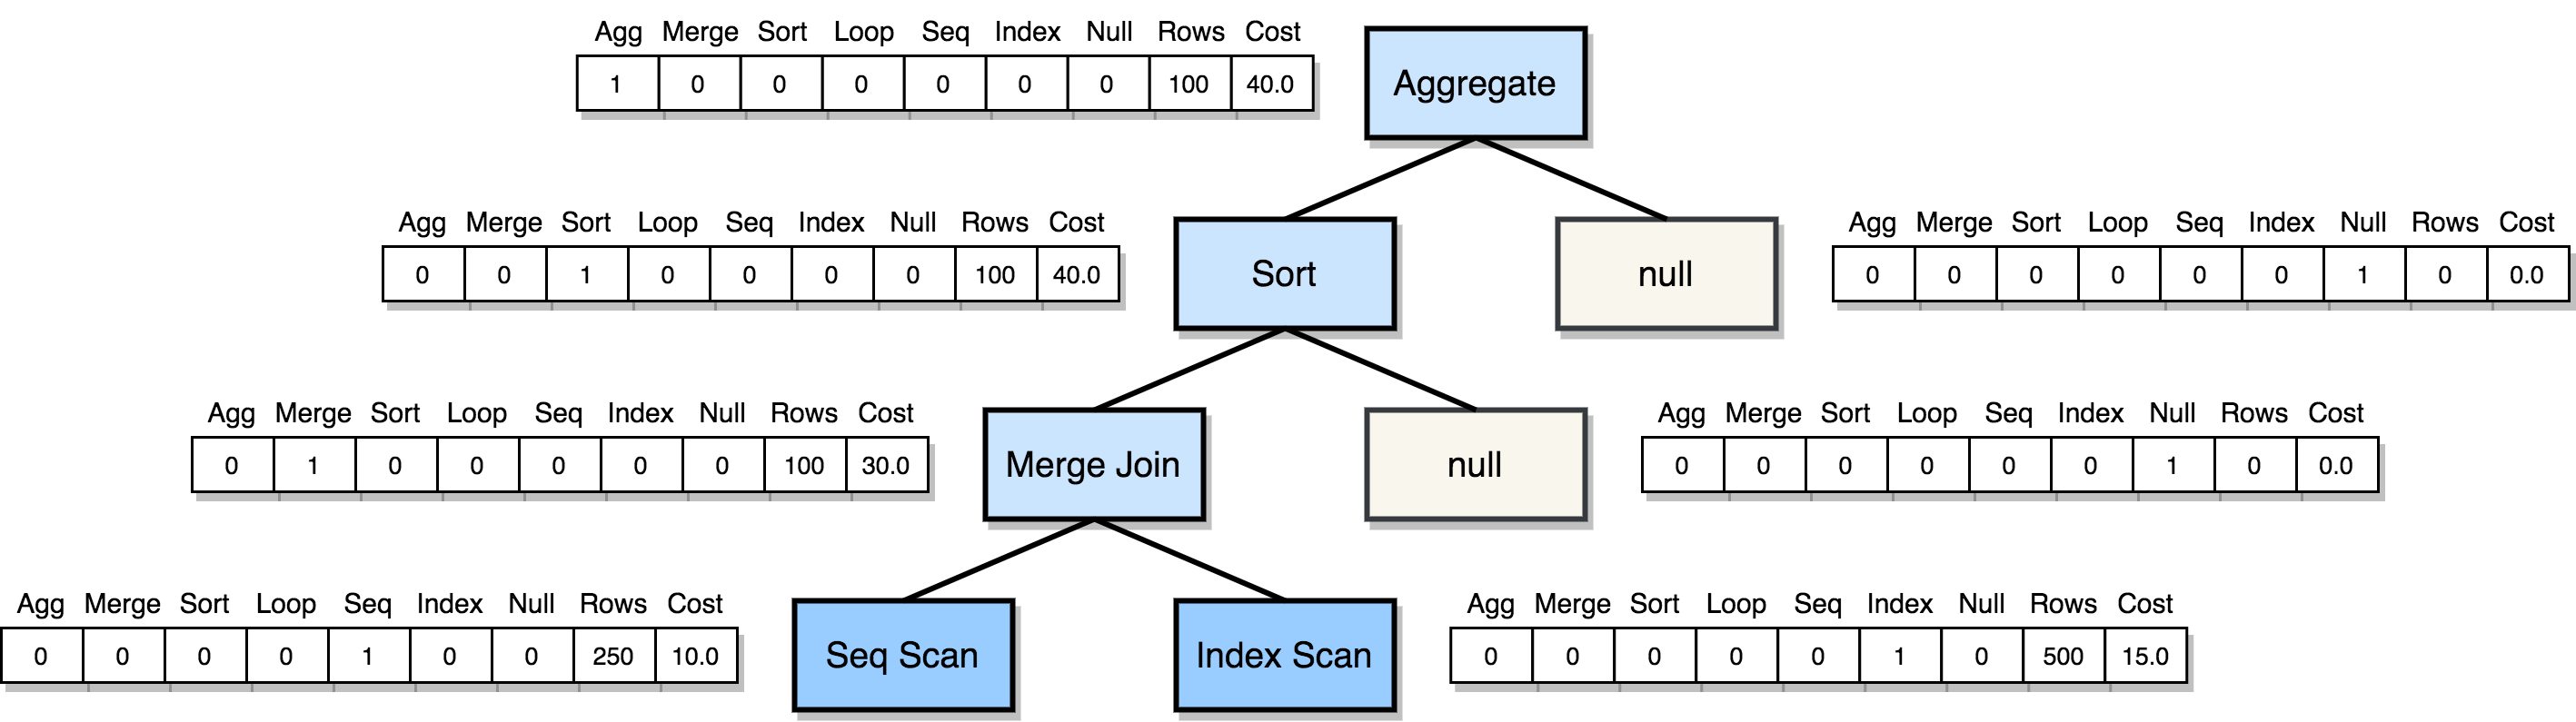
\includegraphics[width=\textwidth]{img/solution/operator_level_featurization.png}
\caption{Operator-level featurization}
\label{fig:operator_level_featurization}
\end{figure}

This featurization approach was first designed in Bao \citep{Marcus2020} and was implemented in Odin to feed the deep learning algorithm described in the following section.

\subsection{Learning Module}

The learning module was devised to have a central role within the system and is responsible for loading pre-trained predictive models to infer the cost of an execution plan having its vector representation as input and building and storing new ones.

The main focal point of Odin is comparing the execution cost of two plans of the same query corresponding to different optimizer configurations. Instead of relying on the optimizer's estimates and cost model for such comparison, Odin models the cost estimation of executing a plan as a regression task as follows:

\begin{quote}
Given a query plan $P$ for a query $Q$ chosen by the optimizer under configuration $C$, the goal is to predict the cost of executing $P$ in terms of execution time.    
\end{quote}

\subsubsection{Predictive Models}

When it comes to predictive models, both traditional algorithms and deep learning approaches should be considered. Using deep neural networks is a computationally heavy task that requires a considerable amount of useful and labeled data. For this reason, more often than not, it might be an overkill approach for more straightforward problems. One simpler approach is to use traditional algorithms, such as linear or tree models to train the predictive model. To make Odin extensible, it supports both types of models allowing to observe whether the use of deep learning is justified.

\paragraph{Traditional Algorithms} 

Odin employs several types of traditional algorithms such as linear regression, a regression variant of Support Vector Machines (\gls{svms}), and Random Forests (\gls{rf}) models for predicting the execution cost of a given plan.

\begin{figure}[ht]
\centering
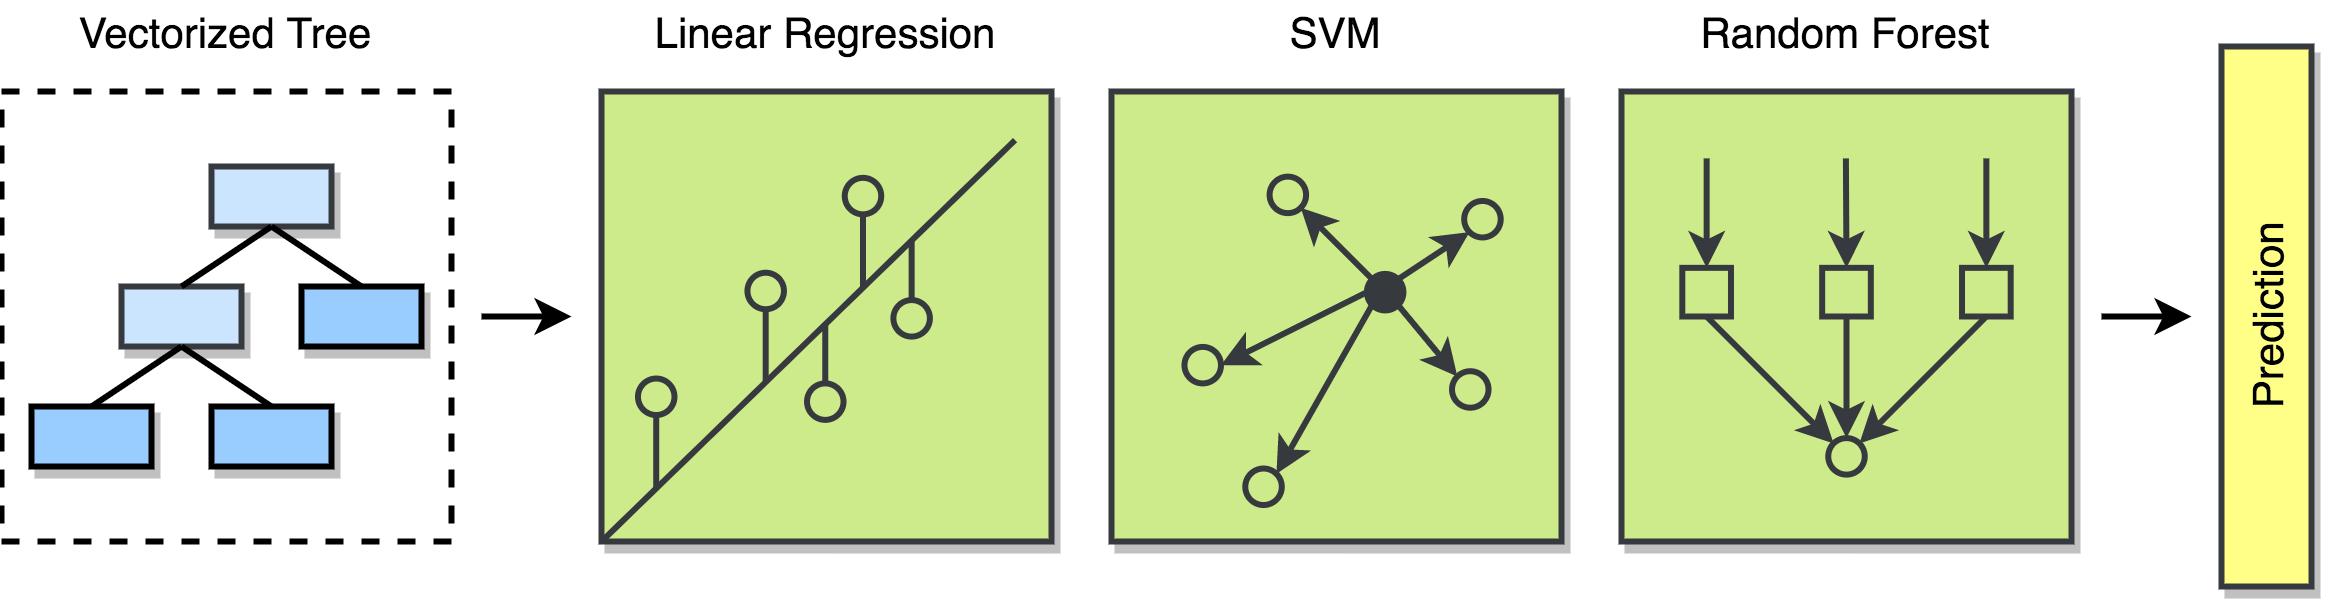
\includegraphics[width=\textwidth]{img/solution/traditional_algorithms.png}
\caption{Traditional machine learning algorithms}
\label{fig:traditional_algorithms}
\end{figure}

As shown in Figure \ref{fig:traditional_algorithms}, for these traditional algorithms, each query plan is featurized into a single vector using the plan-level featurization strategy described earlier.

\paragraph{Tree Convolutional Neural Network} 

A tree convolutional neural network (\gls{tcnn}) is a specialized type of \gls{cnn} that was adapted effectively to query plan trees, providing the ability to automatically learn a large number of filters on a given training data set for query execution time prediction \citep{Marcus2020}.

As in conventional convolutional neural networks, a convolution layer applies several filters to an input tree. The systematic application of the same filter across a query plan allows discovering patterns in the input data. For instance, these filters may look for patterns like pairs of hash joins or an index scan over a small relation.

\begin{figure}[ht]
\centering
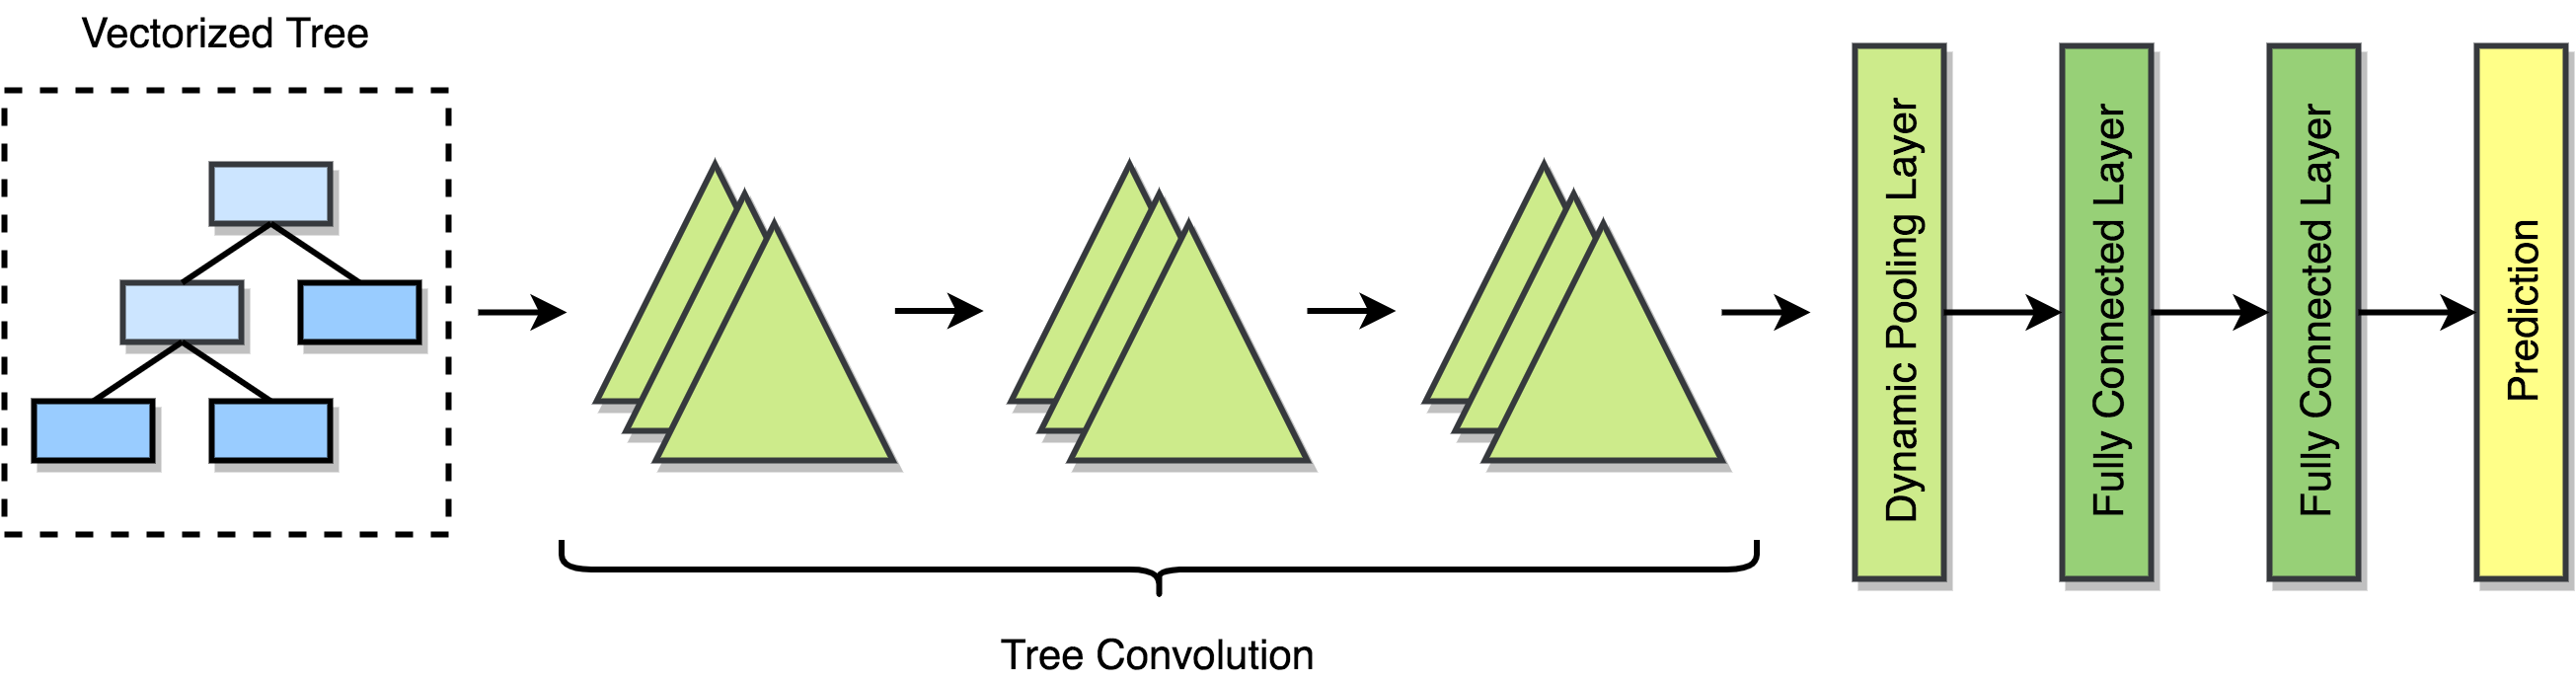
\includegraphics[width=\textwidth]{img/solution/tree_convolutional_neural_network.png}
\caption{Tree convolutional neural network}
\label{fig:tree_convolutional_neural_network}
\end{figure}

Figure \ref{fig:tree_convolutional_neural_network} shows the overall architecture of a \gls{tcnn}. As the output of a tree convolution is another tree, multiple layers of tree convolution filters can be stacked. While the first convolution layer learns simple features (e.g., recognizing a merge join on top of a merge join), the last tree convolution layer learns complex features (e.g., recognizing a left-deep chain of merge joins).

After the query plan tree is passed through a set of tree-based convolutional kernels to extract a query plan's structural information, Odin applies dynamic pooling to gather information over different parts of the tree. Then, a hidden layer and an output layer are added. Finally, two fully connected layers are used to map the pooled vector to predict the execution cost of the given plan.

\subsection{Configuration Tuner}

The configuration tuner is the main module within the system. It has the task of interacting with the PostgreSQL client interface and learning to select the set of strategies that result in the lowest runtime for a particular query. Concerning the actual implementation, this module has two main functions:

\begin{itemize}
    \item Predictive model training: The tuner interacts with the learning module to generate predictive models from a set of \gls{sql} queries that the user specifies as input;
    \item Optimizer configuration tuning: The tuner uses one of the previously generated predictive models to evaluate the best set of strategies for a particular query served as input, returning the result of its execution.
\end{itemize}

\subsubsection{Predictive Model Training}

Besides loading pre-trained predictive models to infer the cost of an execution plan, the configuration tuner module also allows generating and storing new ones. Considering the use of a supervised machine learning approach, Odin relies on historical data to train one of the supported models. Thus, the model training process is based on two basic assumptions:

\begin{itemize}
    \item There is a sample workload (i.e., a set of \gls{sql} queries) representative of the user's total workload;
    \item A traditional query optimizer, such as PostgreSQL, should be used to create valid query execution plans for each query in the sample workload.
\end{itemize}

\begin{figure}[H]
\centering
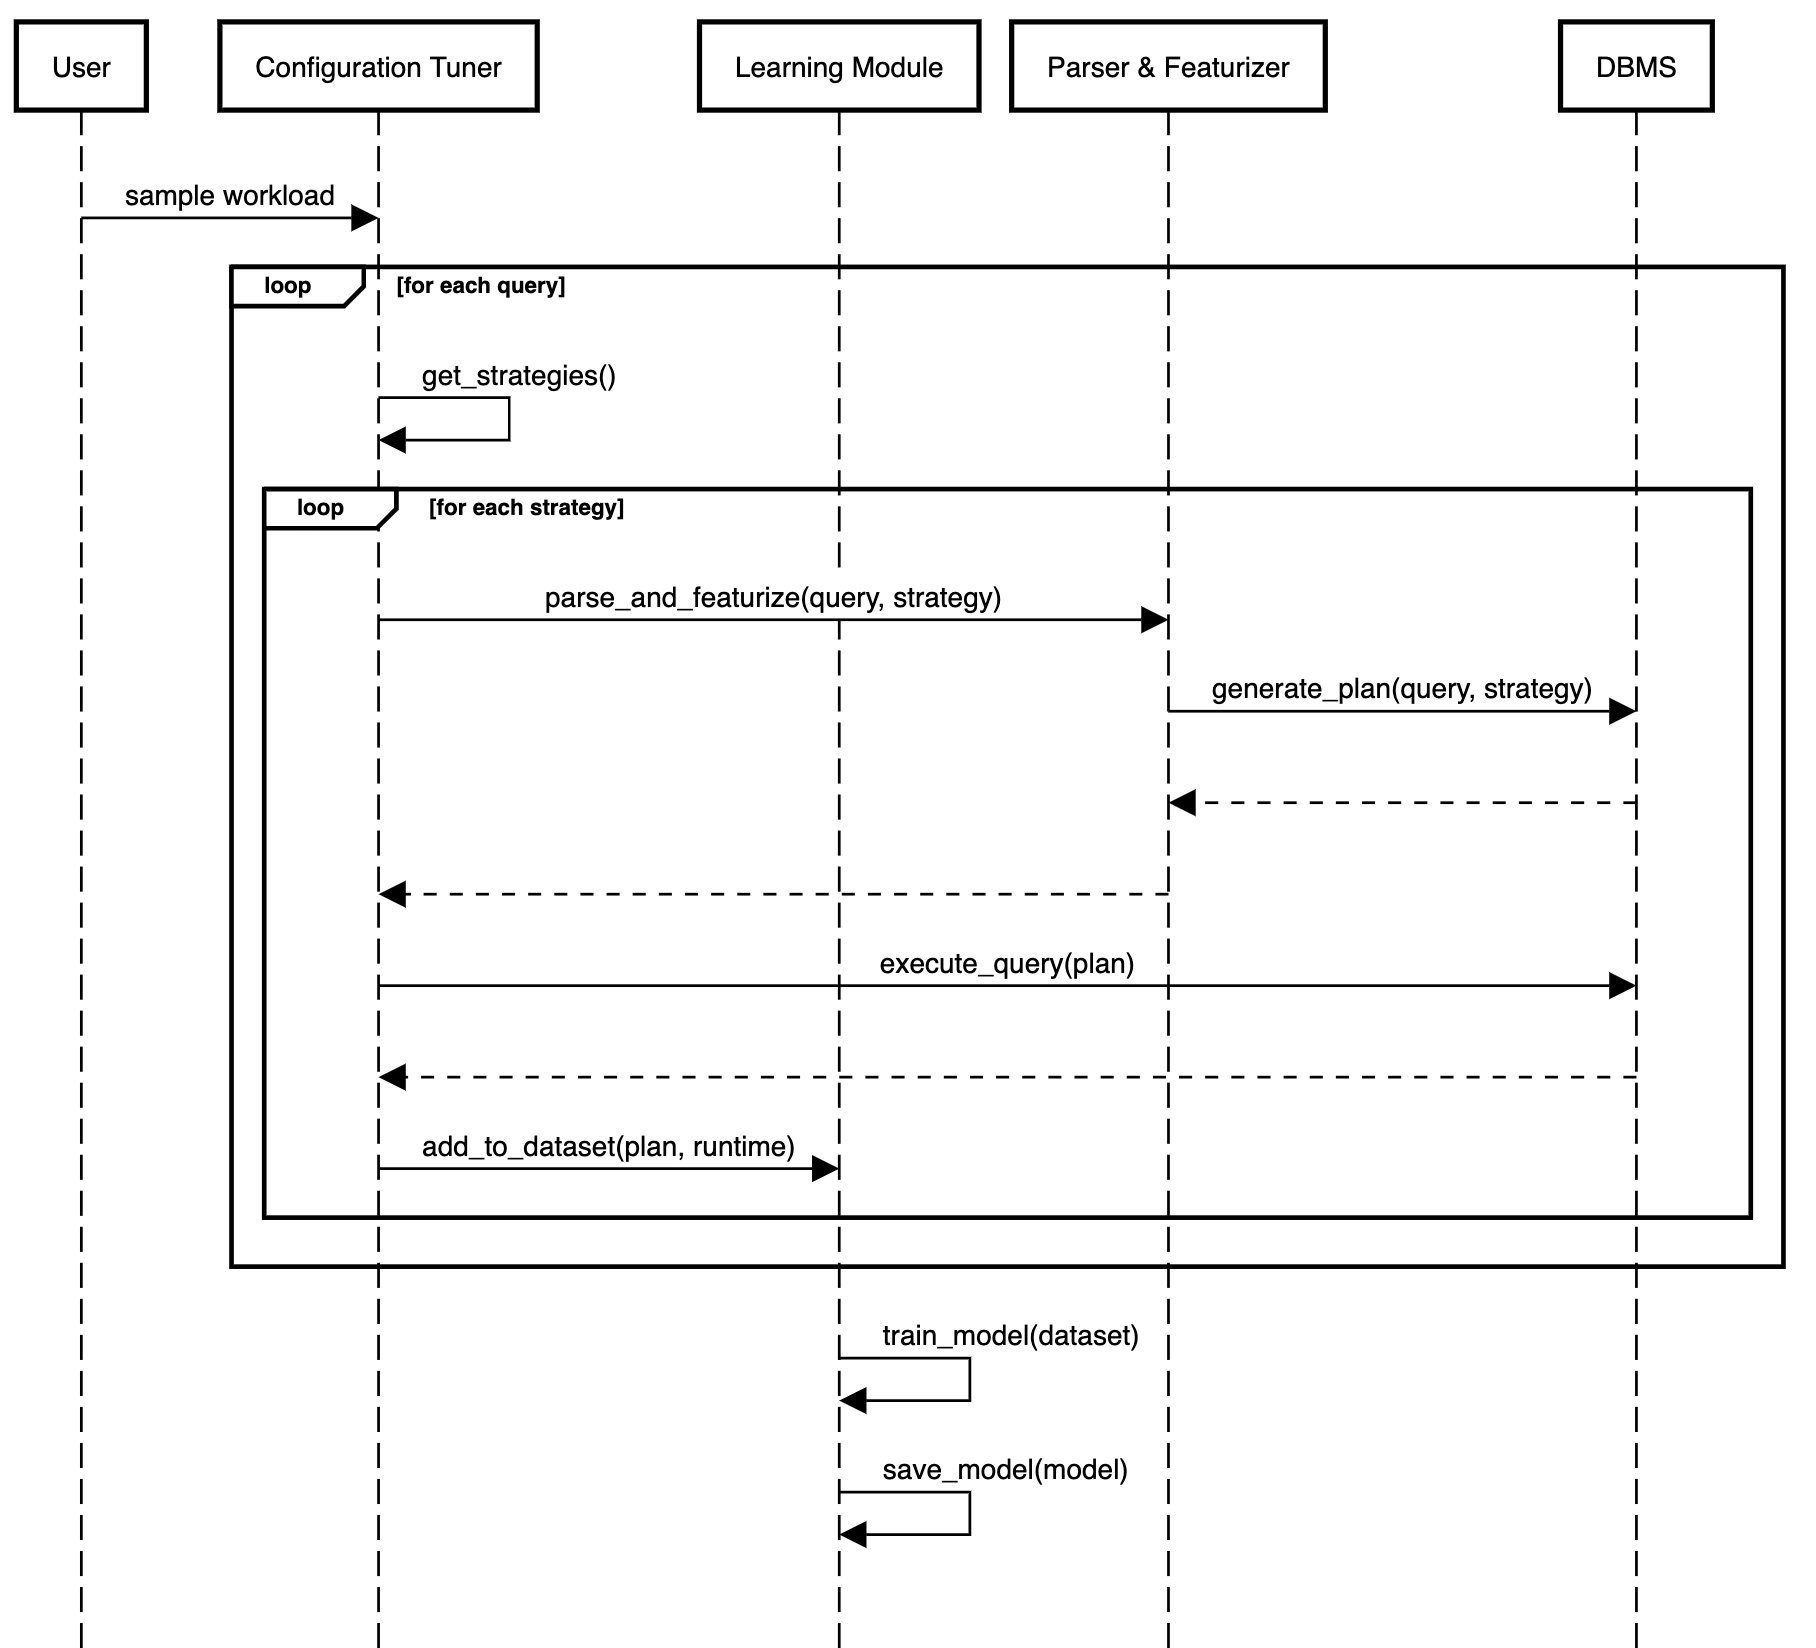
\includegraphics[width=\textwidth]{img/solution/training_sequence_diagram.png}
\caption{Odin's predictive model training}
\label{fig:training_sequence_diagram}
\end{figure}

Figure \ref{fig:training_sequence_diagram} illustrates how this module generates predictive models with the specified sample workload. First, for each query of the sample workload, the configuration tuner generates several plans under different strategy settings. Then, it interacts with the parser and featurizer module to obtain a vectorized representation of the query plan. Finally, it interacts with PostgreSQL to execute each plan and build a model relying on a data set with the plans vectorized representations and their corresponding execution times.

\subsubsection{Configuration Analysis and Selection}

This section discusses the approach to configuration analysis and selection. The problem can be formulated as follows:

\begin{quote}
Given a query $Q$, the goal is to find the set of strategy settings, or configuration $C$, that results in the lowest execution $cost(Q, C)$, where $cost(Q, C)$ is the cost of query $Q$ under configuration $C$.
\end{quote}

\begin{figure}[H]
\centering
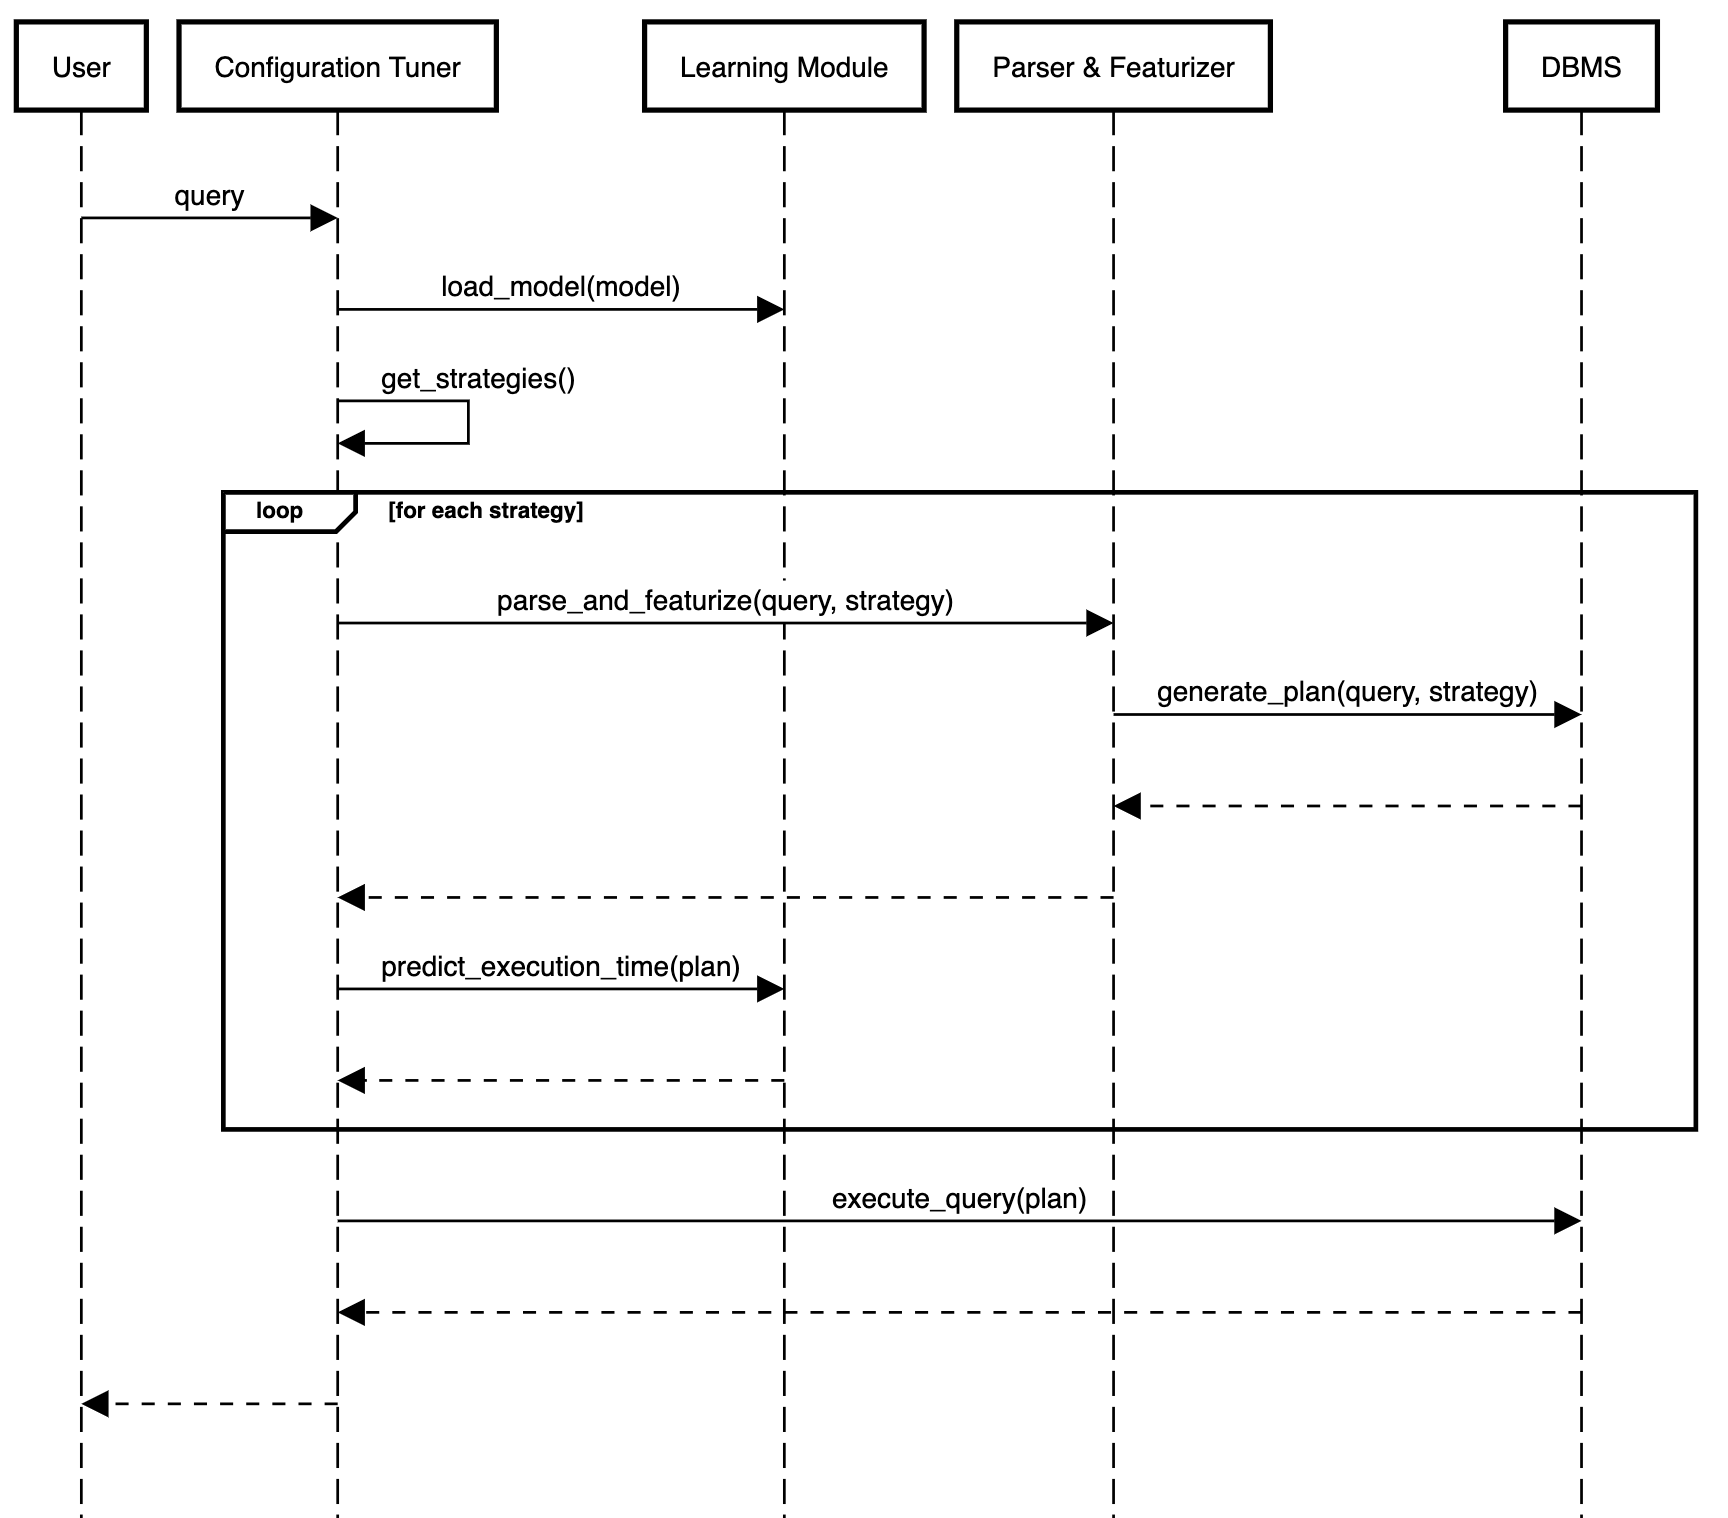
\includegraphics[width=\textwidth]{img/solution/configuration_selection_sequence_diagram.png}
\caption{Odin's configuration analysis and selection}
\label{fig:configuration_analysis_and_selection}
\end{figure}

Figure \ref{fig:configuration_analysis_and_selection} illustrates the steps involved in the process. The configuration tuner starts by interacting with the learning module to load the intended predictive model. Then, it evaluates the effects of disabling certain strategies by interacting with the PostgreSQL client interface to generate query plans under such circumstances. Furthermore, using the cost prediction as its primary input, the configuration tuner sets the configuration with the lowest predicted execution cost following a greedy enumeration algorithm, which is described in further detail in the following section. Finally, it returns the query result to the user.

\paragraph{Plan Enumeration Algorithm}

This section describes how the configuration tuner finds the best configuration for a single query in further detail.

Finding the optimal set of strategy settings requires exhaustive search, which is prohibitively expensive. For this reason, similarly to  index tuners such as \citep{chaudhuri1997}, the plan enumeration algorithm the configuration tuner uses is defined greedily, as illustrated in Figure \ref{fig:greedy_enumeration}. To begin with, a configuration of size $m$ (an arbitrary number where $m \leq k$) must be chosen as a starting point. Then, the algorithm iteratively suggests the rest of the configuration until all $k$ possible strategy settings have been chosen, or no further reduction in execution cost is possible. Each iteration considers all possible choices and adds the one that results in the highest cost reduction.

Since the algorithm requires an arbitrary number \textit{m} as a starting point, it is crucial to find the right balance between the two extremes. On the one hand, if \textit{m = 0}, the algorithm takes a pure greedy approach. On the other hand, if \textit{m = k}, the algorithm is identical to the naive enumeration algorithm. Therefore, the value of \textit{m} relative to \textit{k} reflects the desired degree of completeness of enumeration and is configurable by the user.

\begin{figure}[ht]
\begin{algorithm}[H]
\SetAlgoLined
\DontPrintSemicolon
Let $S$ = the best $m$ configuration using the \textit{naive enumeration algorithm}\\
\Begin{
    1. \textbf{if} $m = k$ \textbf{then} exit\;
    2. Choose a new operator $O$ such that $cost(S \cup \{O\}) \leq cost(S)$ for any choice of\; \hspace{0.3cm} $O \not\in S$\;
    3. \textbf{if} $cost(S \cup \{O_i\}) \geq cost(S)$ \textbf{then exit}\;
      \hspace{0.4cm}{\textbf{else} $S = S \cup \{O_i\}$\;}
    4. \textbf{if} $|S|$ = k \textbf{then exit}\;
    5. \textbf{goto 2}\;
}
$output \longleftarrow$ configuration with minimum cost\;
\caption{Greedy (m, k) enumeration algorithm}
\end{algorithm}
\caption{Odin's greedy enumeration algorithm}
\label{fig:greedy_enumeration}
\end{figure}

\paragraph{Avoiding Regressions}

As shown in Section \ref{sec:preliminary_experiments}, one major concern of enabling or disabling certain strategies is the possibility of causing significant query performance regressions.

To avoid query regressions, we use a constraint that intends to avoid this kind of occurrence. Given a configurable threshold $0 < \alpha < 1$, a plan $P2$ is better than another plan $P1$ if \textit{PredictedCost} $(P2) < (1 - \alpha)$ and more expensive otherwise, where \textit{PredictedCost} is the predicted cost of executing a plan. By default, the value of $\alpha$ is set to 0.15 but can be changed by the user accordingly.
        
\chapter{Performance Evaluation}

    This chapter evaluates the performance of the considered machine learning approach over the ability to improve query runtime.

The evaluation shows that Odin outperforms both approaches that use the query optimizer's cost model to select the best optimizer configuration and the default configuration (i.e., all boolean flags set to true) on two different experimental workloads. 

The experimental analysis is divided into two different parts. Section \ref{sec:experimental_setup}, explains the experimental setup. Section \ref{sec:query_performance_analysis} evaluates the performance against the PostgreSQL query optimizer using different workloads. The major facets of the evaluation are:

\begin{itemize}
    \item Finding whether the presented solution has the ability to improve the overall query runtime, and measure the improvement in query performance;
    \item Inferring the training and inference cost;
    \item Evaluating which type of queries benefit the most from the usage of machine learning to infer the best execution plan;
    \item Interpreting the results and trade-offs between using more traditional machine learning algorithms and deep neural networks;
    \item Hypothesising about how well the approach could be translated into a real-world scenario.
\end{itemize}
    
    \section{Experimental Setup}
    
        \label{sec:experimental_setup}

This section describes all relevant aspects of the PostgreSQL server instance, introduces the benchmarks that were used and presents the methodology for conducting the experimental evaluation.

\subsection{PostgreSQL}
 
All performance experiments were executed on a server with an Intel Core i3-4170 CPU (3.70 GHz) and a total of 4 cores running PostgreSQL 10.12 on Ubuntu 18.04. The system had 16 GB of RAM and a solid state drive of 128 GB.

\begin{table}[H]
\centering
\begin{tabular*}{0.6\textwidth}{p{0.3\textwidth} p{0.3\textwidth}}
\hline
\textbf{Setting}                 & \textbf{Value} \\ \hline
\textit{seq\_page\_cost}         & 1              \\
\textit{random\_page\_cost}      & 4              \\
\textit{cpu\_tuple\_cost}        & 0.01           \\
\textit{cpu\_index\_tuple\_cost} & 0.04           \\
\textit{cpu\_operator\_cost}     & 0.0025         \\ \hline
\end{tabular*}
\caption{PostgreSQL settings overview}
\label{tab:settings}
\end{table}

The experiments were conducted in an out of the box PostgreSQL server, meaning that every planner constants of the optimizer were set to the default values. Table \ref{tab:settings} summarizes the used settings. The planner's estimate of the cost of a disk page sequential fetch was set to 1. The planner's estimate of the cost of a non-sequentially-fetched disk page was set to 4. Furthermore, the planner's estimate of the cost of processing each row during a query, processing each index entry during an index scan and processing each operator or function executed during a query were set to 0.01, 0.04 and 0.0025 respectively. Finally, the planner's assumption about the disk cache's effective size available to a single query was set to 4 GB.

\subsection{Workloads}
\label{sec:workloads}

Two separate workloads were considered in the experiments: (1) the TPC-H benchmark \citep{tpch} and (2) the Join Order Benchmark (\gls{job}) \citep{JOB}. The precise details are outlined in Table \ref{tab:workloads} below.

\subsubsection{TPC-H Benchmark}

The Transaction Processing Performance Council (TPC) benchmark TPC-H has been extensively used by database software and hardware vendors and the research community. It intends to evaluate the performance of several decision support systems that process large volumes of business data and execute queries with a high degree of complexity. TPC-H comes with various data set sizes to test different scaling factors. It consists of 22 standard query templates, where each query asks a business question and includes the corresponding query to answer the question.

\subsubsection{Join Order Benchmark}

While the standard benchmarks like TPC-H have proven their value for evaluating query engines, they are not valuable benchmarks for the cardinality estimation component. The reason is that they use data generators based on the same simplifying assumptions that query optimizers make (i.e., uniformity, independence, the principle of inclusion) to be able to scale the benchmark data efficiently \citep{Leis2015}.

Instead of using a synthetic data set, the Join Order Benchmark is a workload based on the Internet Movie Database, a real-world data set containing plenty of information about movies and related facts about actors, directors, production companies, among others. It provides a total of 113 analytical SQL queries, which have between 3 and 16 joins, with an average of 8 joins per query.

For the \gls{job} benchmark, we use a further extension of 24 additional queries \citep{Marcus2018a}. These queries were designed to test systems trained on regular \gls{job} queries. They use the same relations but have very different semantics.

\begin{table}[H]
\centering
\begin{tabular*}{0.9\textwidth}{p{0.25\textwidth} p{0.30\textwidth} p{0.35\textwidth}}
\hline
\textbf{Workload} & \multicolumn{1}{l}{\textbf{Database Size (GB})} & \multicolumn{1}{l}{\textbf{Query Templates (\#)}}   \\ \hline
JOB       & 3.6       & 137                       \\
TPC-H 10    & 10        & 22                        \\
TPC-H 25    & 25        & 22                        \\ \hline
\end{tabular*}
\caption{Workloads statistics overview.}
\label{tab:workloads}
\end{table}

For the TPC-H benchmark, two different scale factors were considered namely, 10 and 25 (i.e., 10 GB and 25 GB). Ten queries were generated  for each one of the 22 standard query templates, making a total of 220 queries. On the other hand, the \gls{job} used a snapshot of data from the Internet Movie Database (IMDb) with 3.6 GB and a total of 137 unique queries.

\subsection{Modeling}

To build and evaluate the predictive models, training and test data sets were derived from the aforementioned workloads. Since the goal is to improve query runtime by recommending the optimal configuration on a per-query basis, execution plans under different configurations for each query following the predictive modeling process were generated. They are outlined in Figure \ref{fig:training_sequence_diagram}. The features from those query plans were extracted (e.g., optimizer estimates and operators involved) and used the actual query runtime as the training labels.

To keep the overall experimentation under control,  a limit of 5 minutes execution time per query for the \gls{tpch} 10 GB database was enforced. Within the \gls{tpch} 25 GB, the execution time limit was set to 15 minutes. Whenever the limit is reached, the query runtime is set as double the timeout value in the data set.

\subsection{Metrics and Validation}

To evaluate the Odin's ability to reduce query runtime, a 5-fold cross-validation method was considered. Within each fold, the models were trained on 80\% of the queries. Their ability to choose the best configuration was evaluated on the remaining 20\%. A comparison between the  learned approach against two different baselines is provided, namely:

\begin{itemize}
    \item The default optimizer configuration, where all boolean flags are set to true by default;
    \item The configuration tuner, where decisions are made directly based on cost estimates returned by the optimizer cost model instead of a machine learning model.
\end{itemize}
    
    \section{Query Performance Analysis}
    
        \label{sec:query_performance_analysis}

This section evaluates the effectiveness of the solution over the ability to recommend optimizer configurations and improve query runtime as a result. It starts with a predictive model comparison between different types of algorithms and the feasibility of using deep learning approaches in this type of problem. It then evaluates whether the machine learning-based approach can improve the overall query runtime or not compared to the query optimizer by itself.

For every experiment that considers the greedy enumeration algorithm described in the previous chapter, the arbitrary number \textit{m} that defines the initial configuration size was set to a default value of 2.

\subsection{Predictive Model Comparison}

One of the key goals of the experiments was to evaluate the effectiveness of different types of machine learning algorithms to predict query runtime. This comparison is based on how well the different predictive models could be employed in the configuration selection algorithm and observe to what extent they could improve the overall query performance.

\subsubsection{Traditional Algorithms}

Initially, the Random Forest and Support Vector Regression models were evaluated, while treating the problem as a regression task. The Linear Regression model was discarded altogether due to low accuracy during the model validation phase.

\begin{figure}[H]
  \begin{subfigure}[t]{0.5\textwidth}
    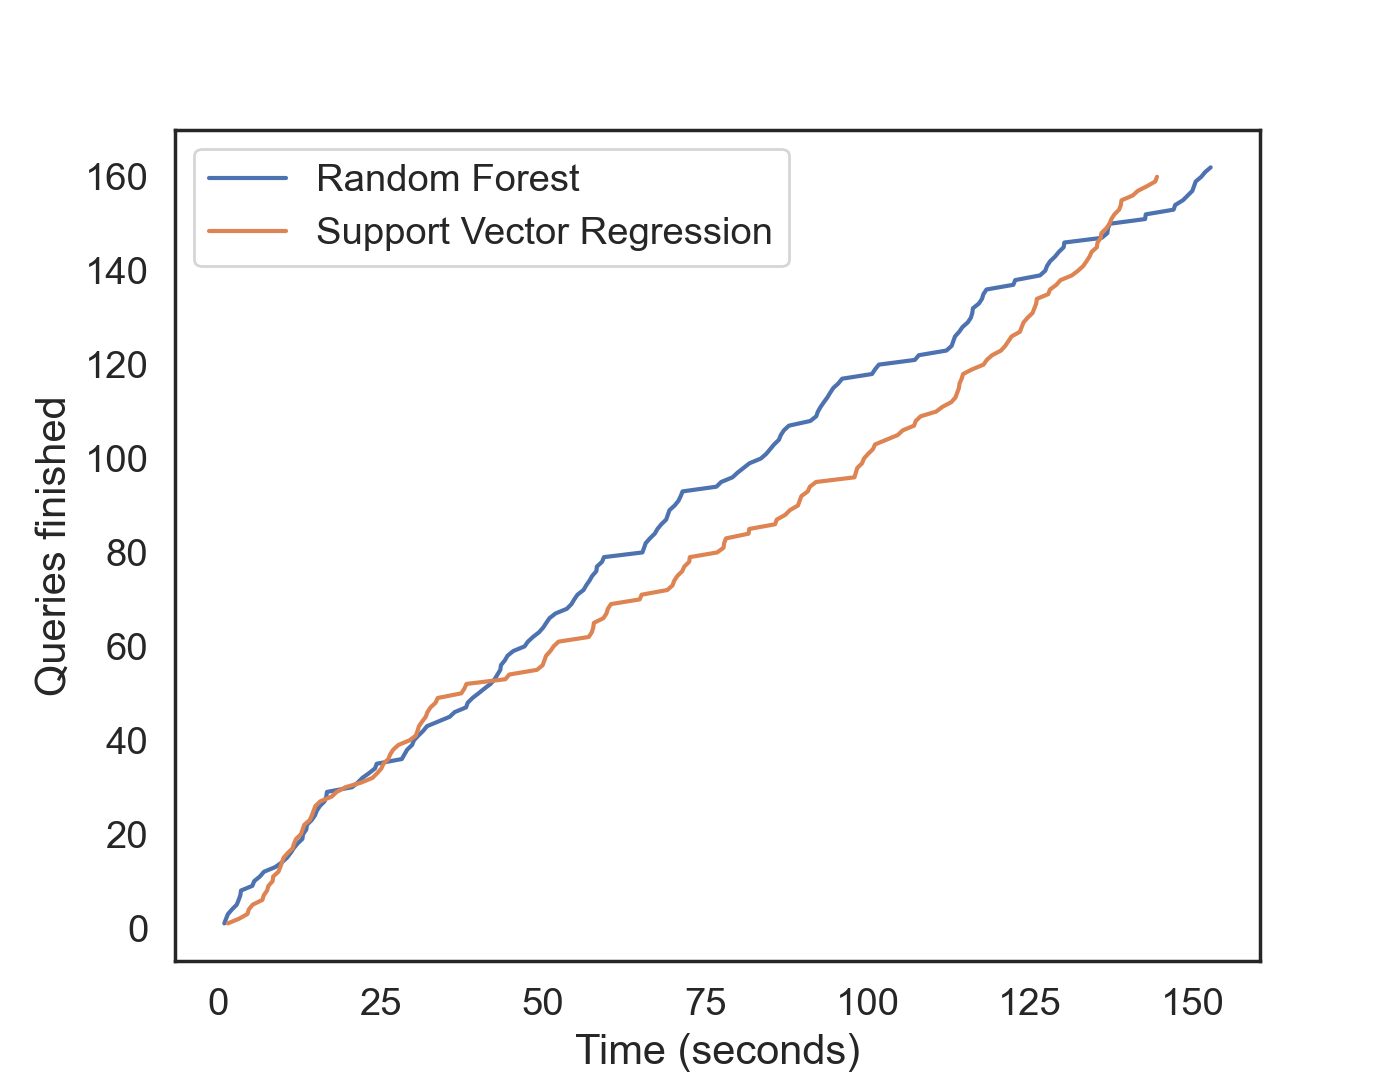
\includegraphics[width=\textwidth]{img/performance_evaluation/tpch_models_comparison.png}
    \caption{\gls{tpch} workload}
  \end{subfigure}\hfill
  \begin{subfigure}[t]{0.5\textwidth}
    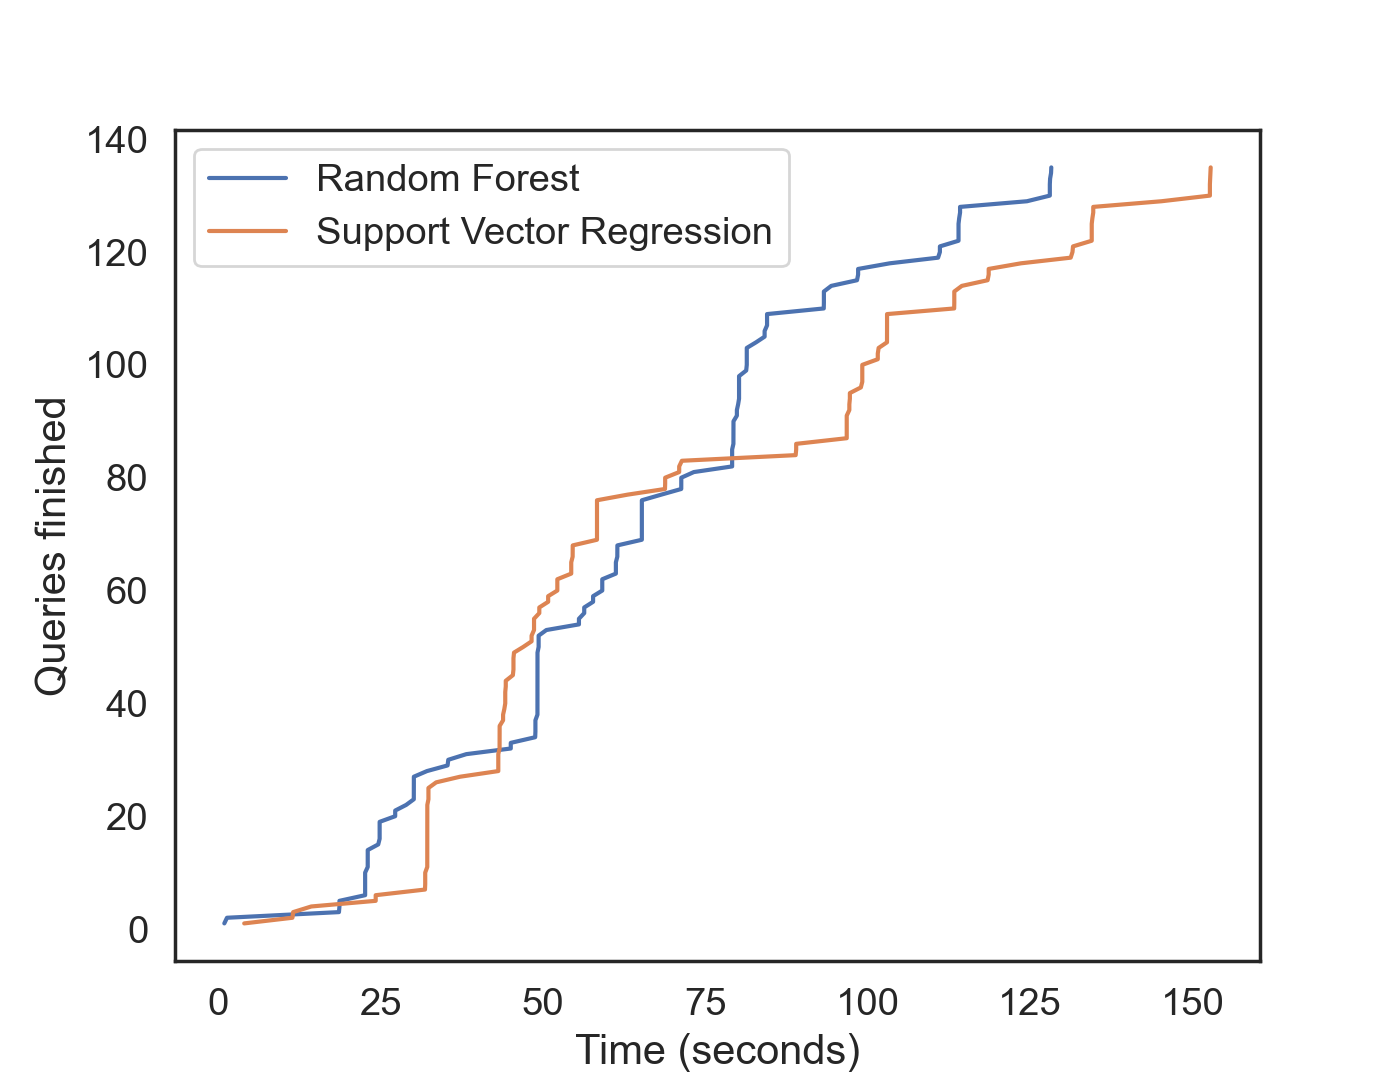
\includegraphics[width=\textwidth]{img/performance_evaluation/job_models_comparison.png}
    \caption{\gls{job} workload}
  \end{subfigure}
  \caption{Traditional predictive model comparison for the \gls{tpch} and \gls{job} workloads}
  \label{fig:model_comparison}
\end{figure}

Figure \ref{fig:model_comparison} presents a quantitative comparison between the two. Each plot shows the performance curves for the \gls{tpch} workload and the JOB workload. They represent the overall query runtime over a set of queries that were not part of the training data set. It is possible to observe that, for the \gls{tpch} workload, Support Vector Regression outperforms the Random Forest model in the overall execution runtime even though the runtime of the latter flowed at a steadier pace over time. For the \gls{job} workload, Random Forest outperforms Support Vector Regression, meaning that it made better execution plan choices for a short sample of queries, resulting in a meaningful reduction in the overall execution runtime.

\subsubsection{Tree Convolutional Neural Networks}

Even though the two algorithms mentioned above can offer more interpretability and simplicity, in certain scenarios, deep neural networks can increase adaptability at the cost of needing more quality and quantity of data. To determine if this was the case, further experiments were carried out using specialized tree convolutional neural networks.

\begin{figure}[H]
\centering
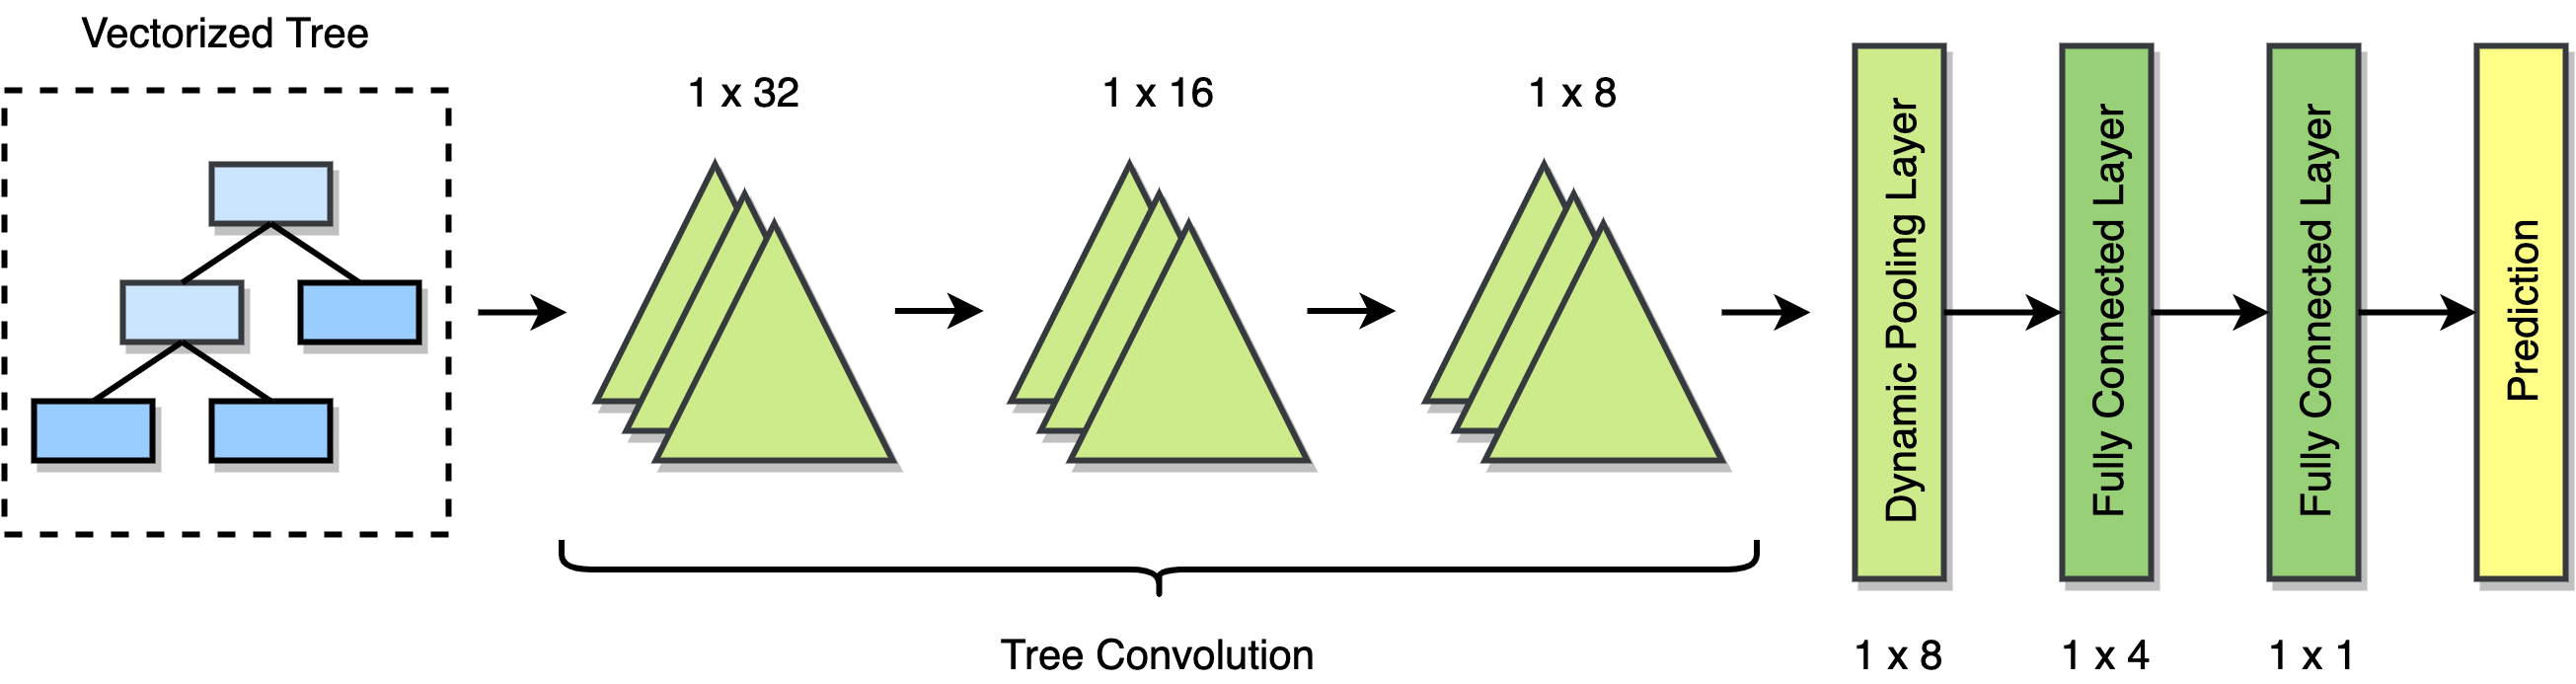
\includegraphics[width=\textwidth]{img/performance_evaluation/tcnn_architecture.png}
\caption{Tree convolutional neural network experimental architecture}
\label{fig:tcnn_experimental_architecture}
\end{figure}

As shown in Figure \ref{fig:tcnn_experimental_architecture}, the used architecture employs three layers of tree convolution, with output dimensions (32, 16, 8), followed by a dynamic pooling layer and two linear layers with output dimensions (4, 1). The Rectified Linear Unit (ReLU) activation functions and layer normalization between each layer were considered. Training is performed with SGD and is ran until 100 epochs elapsed.

To begin with, in contrast to the previous experiments with more traditional algorithms, the number of queries generated per template was increased for the \gls{tpch} workload. Increasing the number of queries per template from 10 to 40, making almost 800 queries would make the training process more robust.

\begin{table}[H]
\centering
\begin{tabular*}{0.5\textwidth}{p{0.25\textwidth} p{0.25\textwidth}}
\hline
\textbf{Batch Size}              & \textbf{\gls{rmse} (ms)}  \\ \hline
4                                & 91 796                   \\
8                                & 93 678                   \\
16                               & 94 099                   \\ \hline
\end{tabular*}
\caption{\gls{rmse} for different batch sizes}
\label{tab:tcnn_results_1}
\end{table}

Table \ref{tab:tcnn_results_1} shows the training results of different batch sizes after 100 epochs elapsed. Even though the training process flowed at a nice and steady pace, the final \gls{rmse}s are not satisfactory. At this point, it is worth considering whether increasing the original data set could lead to better results and proceeded with two additional experiments, which would be done separately:

\begin{itemize}
    \item Increase the database size from 10 GB to 25 GB and evaluate its impact in training;
    \item Double the number of queries per template from 40 to 80 to increase the size of the data set.
\end{itemize}

\begin{table}[H]
\centering
\begin{tabular*}{0.8\textwidth}{p{0.4\textwidth} p{0.4\textwidth}}
\hline
\textbf{Scenario}                & \textbf{Average \gls{rmse} (ms)}  \\ \hline
Scaled-up database of 25 GB      & 394 672                     \\
80 queries per template                   & 84 401                      \\ \hline
\end{tabular*}
\caption{\gls{rmse} for different scenarios during \gls{tcnn} training}
\label{tab:tcnn_results_2}
\end{table}

As shown in Table \ref{tab:tcnn_results_2}, the results with the new scaled-up database were not much different. While it was expectable that the average query runtime would be higher (i.e., 539 331 ms), the average \gls{rmse} was also higher than desirable (i.e., 394 672 ms) in comparison.

For the second experiment, doubling the number of queries per template from 40 to 80 resulted in slightly better results. The average \gls{rmse} of 84 401 ms roughly translates into a decrease of almost 10 seconds in comparison to the experiment with a smaller data set. This leads to conclude that increasing the number of queries per template would help to achieve better results. However, the cost of generating a more extensive data set would be impractical in real-world scenarios.

\subsection{Optimizer Comparison}

Going into more detail in the experimental campaign, the Random Forest model performance was evaluated against the out-of-the-box PostgreSQL query optimizer. With this in mind, a comparison against two different baselines was considered:

\begin{itemize}
    \item The first one refers to the default optimizer configuration where the PostgreSQL optimizer has all settings enabled by default;
    \item The second one represents the enumeration algorithm that makes decisions directly based on cost estimates returned by the optimizer's cost model in contrast to the learned solution that makes its decisions based on the Random Forest model predictions.
\end{itemize}

The idea was to infer whether the same results could be obtained and discard the overhead of collecting execution data and train a machine learning model entirely.

\begin{figure}[H]
    \begin{subfigure}[t]{0.5\textwidth}
    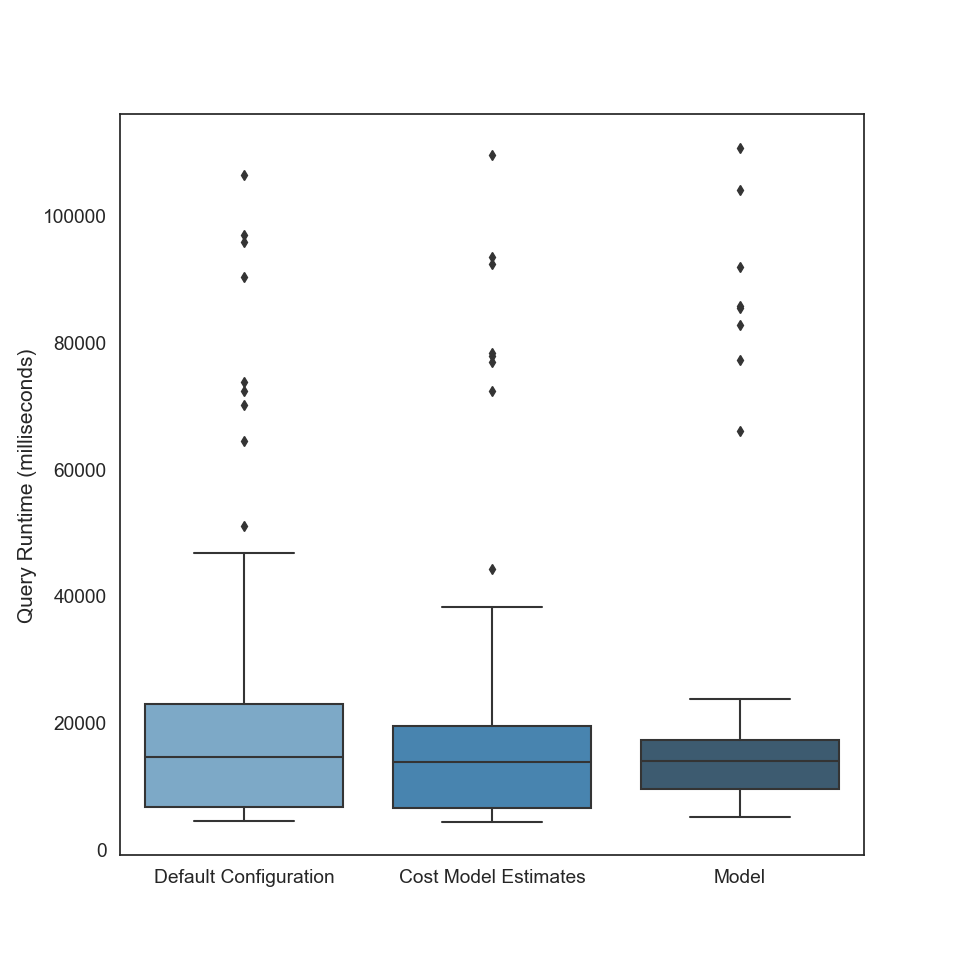
\includegraphics[width=\textwidth]{img/performance_evaluation/tpch_rf_optimizer_comparison.png}
    \caption{\gls{tpch} workload}
    \label{fig:tpch_boxplot}
    \end{subfigure}\hfill
    \begin{subfigure}[t]{0.5\textwidth}
    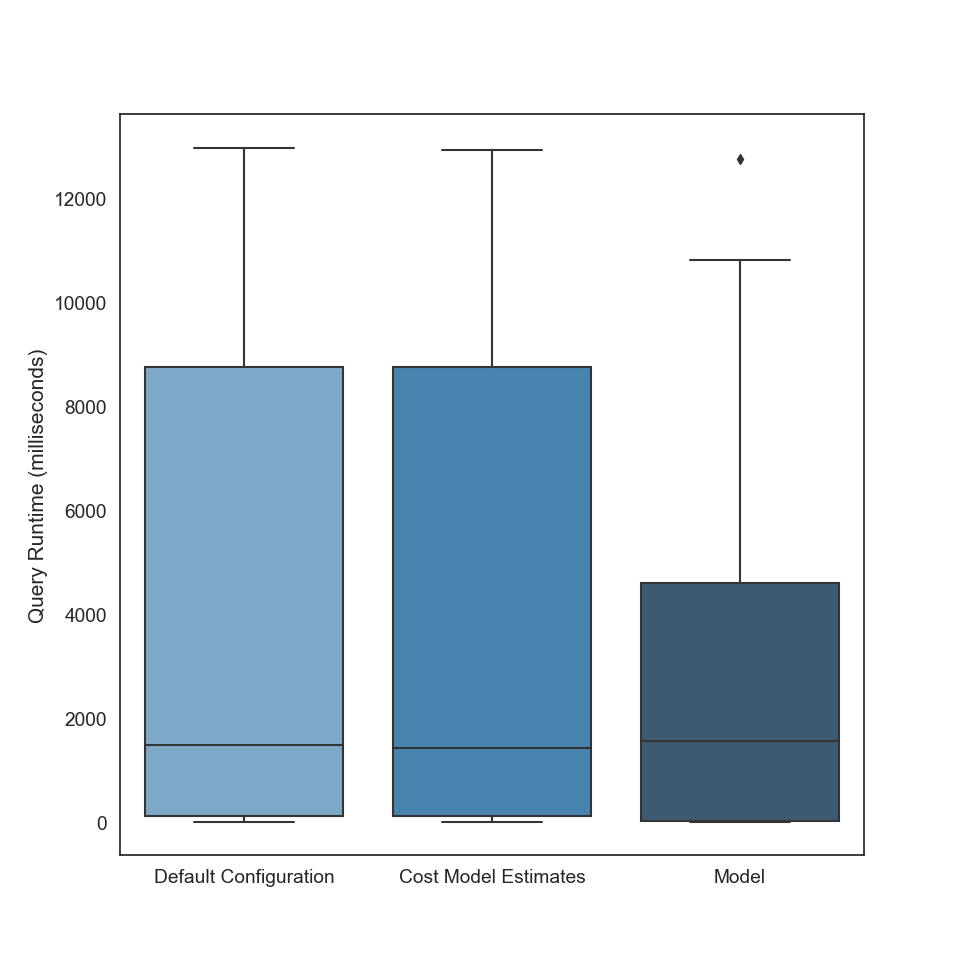
\includegraphics[width=\textwidth]{img/performance_evaluation/job_rf_optimizer_comparison.png}
    \caption{\gls{job} workload}
    \label{fig:job_boxplot}
    \end{subfigure}
    \caption{Query runtime comparison between the three approaches} 
    \label{fig:boxplot}
\end{figure}

Figure \ref{fig:boxplot} summarizes the results using the three different approaches. Using cost model estimates for the \gls{tpch} queries resulted in a slight improvement over the default configuration, but the learned model still outperformed both. On the other hand, for the \gls{job} queries, using the cost model estimates and leaving the optimizer settings to the default configuration, resulted in nearly the same execution runtime distribution, whereas the learned approach surpassed both.

\subsubsection{Operator Type Analysis}

Evaluating the proposed solution on a query-level basis allowed to delve into the model's optimizer settings configuration choices. Throughout the experimental evaluation, the chosen configuration for each one of the assessed queries was recorded. As a result, it is possible to infer the number of times a given operator type was selected to be disabled and discover specific patterns between the two workloads. It is important to note that the choice of operators is not mutually exclusive, meaning that a given configuration may simultaneously include two or more operators.

\begin{figure}[H]
\begin{subfigure}[t]{\textwidth}
    \centering
    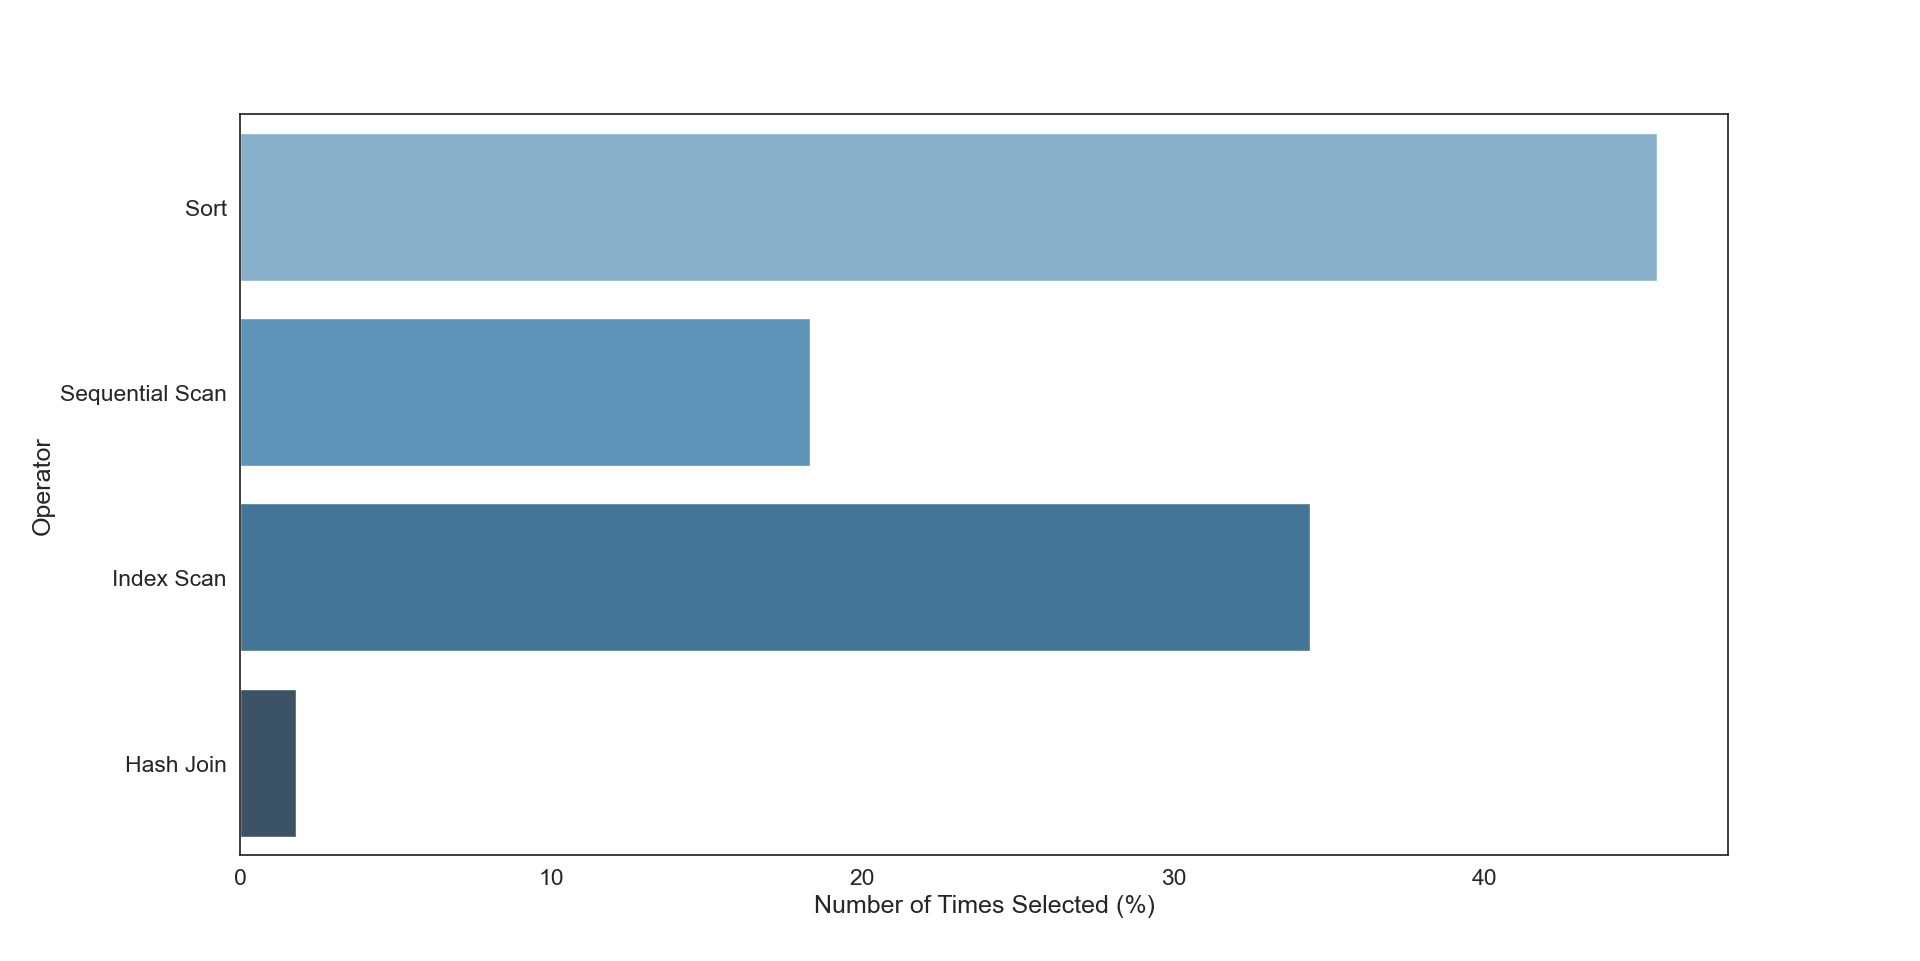
\includegraphics[width=0.8\textwidth]{img/performance_evaluation/tpch_operator_analysis.png}
    \caption{\gls{tpch} workload}
    \label{fig:tpch_operator_analysis}
\end{subfigure}
\begin{subfigure}[t]{\textwidth}
    \centering
    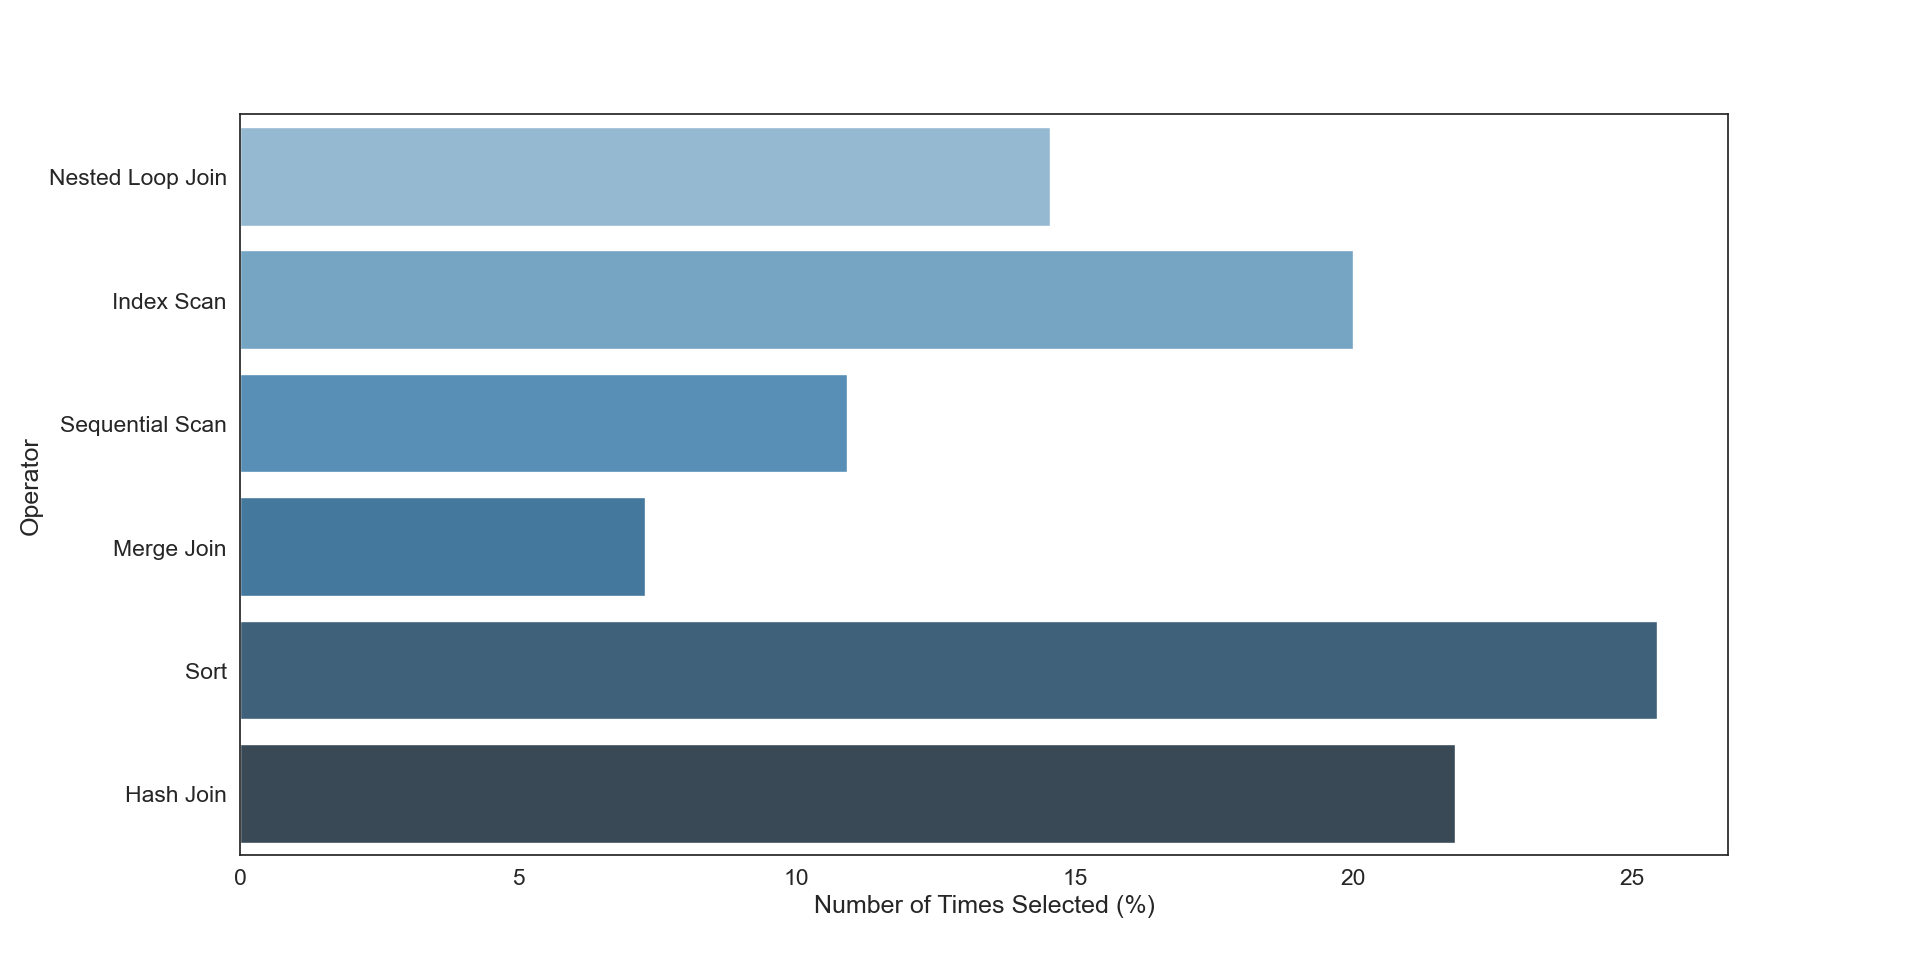
\includegraphics[width=0.8\textwidth]{img/performance_evaluation/job_operator_analysis.png}
    \caption{\gls{job} workload}
    \label{fig:job_operator_analysis}
\end{subfigure}
\caption{Number of times an operator was selected to be disabled}

\end{figure}

Figure \ref{fig:tpch_operator_analysis} shows that only four operator types are dismissed throughout the experimental evaluation for the \gls{tpch} workload, with the \textit{sort} being the most frequent one. The choice of disabling the \textit{index scan} could be explained by the absence of indices, while \textit{sequential scan} tends to be one of the most costing types of operations. Bear in mind that disabling each of these operators does not necessarily mean that it was the right decision, as there are some cases where performance regressions happen.

Similar to the previous one, Figure \ref{fig:job_operator_analysis} illustrates which types of operators are discarded throughout the experiments for the \gls{job} workload. Notice how two additional join operator types are now considered compared to the \gls{tpch} workload. It can be easily explained by the fact the most of the \gls{job} queries have an average of 8 joins per query, as mentioned before.

\subsubsection{Query Type Analysis}

This section evaluates the difference in performance relative to the default set of settings for each query. To get more insight about which type of queries can benefit the most by using machine learning, the query performance for each of the executed \gls{tpch} queries in the experimental phase was analyzed.

\begin{figure}[H]
\centering
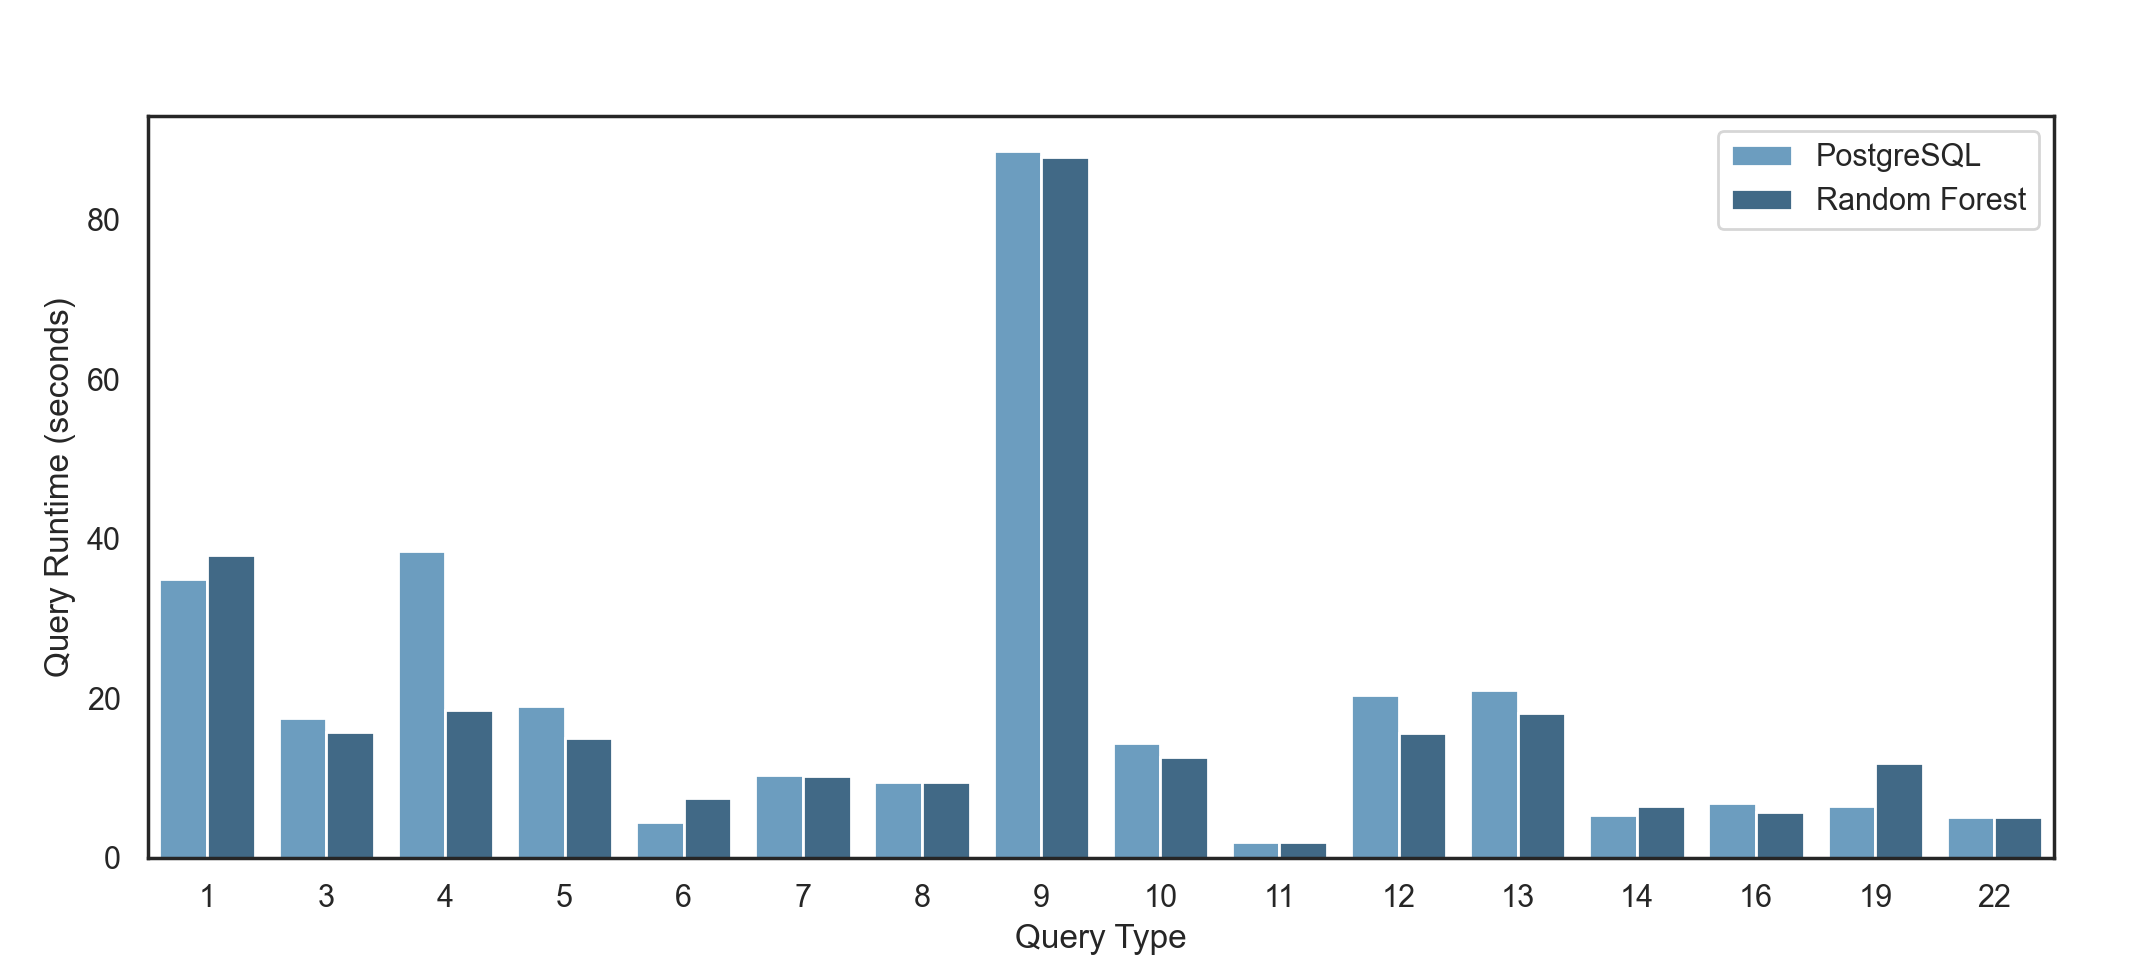
\includegraphics[width=\textwidth]{img/performance_evaluation/tpch_query_analysis.png}
\caption{Runtime difference per query between PostgreSQL and Random Forest for the \gls{tpch} workload}
\label{fig:tpch_query_analysis}
\end{figure}

Figure \ref{fig:tpch_query_analysis} shows the difference in runtime between the plan chosen by our learned approach and the PostgreSQL default one. Of the 16 \gls{tpch} queries shown above, the Random Forest algorithm only incurs regressions on five, and these regressions are all under 5 seconds. The remaining 11 see performance improvements of up to 20 seconds. While the learned algorithm does not always choose the best plan compared to the default configuration, it comes close to almost every query.

Please note that a specific threshold was enforced to avoid unwanted significant query performance regressions, set to 0.15 by default. Increasing the regression threshold would help to decrease the probability of such regressions at the cost of decreasing the probability of potential query performance improvements.

\subsection{Inference and Training Overhead}

A significant concern with any application of machine learning is training time overhead. Across all workloads, generating the data set is the procedure that takes longer since it requires that a single query run multiple times with different configurations to make the training process more robust. As a result, the training process will better capture the impact of different settings on the final query execution runtime.

For the \gls{tpch} workload:

\begin{itemize}
    \item Generating the data set takes about 16.4 hours, using ten queries per template;
    \item Training the model takes up to 12 seconds;
    \item Inferring the best plan had a maximum increase of 114 milliseconds on planning time compared to the out-of-the-box PostgreSQL optimizer.
\end{itemize}

As for the Join Order Benchmark:

\begin{itemize}
    \item Generating the data set takes about 25 minutes;
    \item Training the model takes up to 13 seconds;
    \item Inferring the best plan had a maximum increase of 613 milliseconds on planning time compared to the out-of-the-box PostgreSQL optimizer.
\end{itemize}

Since analytic queries generally run for many seconds or minutes, an optimization time of a few milliseconds may be acceptable in most applications. Seeing that generating the data set may take up much time, even for a relatively small data set, this work further proposes new considerations that could be taken into account when applying machine learning-based query optimization solutions in a real-world scenario.

\subsection{Translating Into a Real-World Scenario}

Most machine learning algorithms focus on batch training, meaning that all training data is available beforehand. More recent techniques allow the training process to be done incrementally while a continuous stream of data is made available over time. Stream learning models are created incrementally and are updated continuously. Learning incrementally from a mini-batch of instances would be essential to out-of-core learning in query optimization. It would take away the concern of having queries execution history.

In a real-world scenario, changes in data distribution may harm learning. Using an adaptive sliding window method would allow the algorithms to be more robust to concept drift changes in dynamic environments such as query optimization. The general idea is to keep metrics and statistics from a window of variable size. The algorithm decides the window's size by cutting the window at different points and analyzing the average of a particular metric over these two windows. If the difference between the two averages surpasses a pre-defined threshold, change is detected, and all data before that time is discarded.

In the context of stream learning, another concern is evaluating the performance of a learned model. It can be measured using two predominant techniques:

\begin{itemize}
    \item Using a holdout evaluation where the performance evaluation happens periodically, at which moment the evaluator will test the learner's performance on a test set, formed by yet unseen queries, which will be used to evaluate performance, but not to train the model;
    \item Using a prequential evaluation where each data sample serves two purposes. Each query is analyzed sequentially, in order of arrival, and becomes immediately inaccessible. This method involves using each sample to test the model (i.e., make a prediction) and then use the same sample to train the model. By doing this, the model is always tested on samples that it has not seen yet.
\end{itemize}

Being conceived to serve as a platform to encourage the democratization of stream learning research, \textit{scikit-multiflow} \citep{montiel2018} is a framework that provides multiple state-of-the-art learning methods, data generators, and evaluators for different stream learning problems. It builds upon popular open-source frameworks, including \textit{scikit-learn} \citep{pedregosa2011}, in which our solution is built upon.

\chapter{Conclusions}

    This dissertation addresses the viability of using machine learning in query optimization by proposing a middleware layer that can be used on top of a conventional relational database.

The solution is based on the client interface of the underlying database extending it with machine learning capabilities to select the best set of strategy settings on a per-query basis. The prototype was built around three different modules with distinct concerns that interact with one another to leverage machine learning techniques to improve optimizer settings recommendation quality with minimal changes to state-of-the-art database systems. Since it extends the \gls{dbms} interface and has minimal impact on the database clients, it can be further extended with new features to enhance query optimization even more.

The prototype implementation was built on top of PostgreSQL. It was tested using two different benchmarks to evaluate the benefits and the overall cost of adding machine learning guarantees to the underlying query optimizer. The results have shown us that, when using the \gls{tpch} benchmark, a read-intensive workload, the overall query runtime decreased by 3\%, while with \gls{job}, a real-world data set with an average of 8 joins per query the impact was as far as 19\%. In conclusion, the results have shown that integrating learned models represents a candidate way of comparing the execution cost of different plans and results in higher accuracy than using cost model estimates or keeping the optimizer strategy settings to their default values.

\section{Future Work}

One of the main goals for this dissertation was to create a middleware that would be applied to any relational database by leveraging readily available mechanisms in most database systems.

The prototype was implemented on top of PostgreSQL. However, it intended to test the solution on top of other state-of-the-art database systems. In short, a new research question would be to investigate whether the solution can obtain the same machine learning capabilities and results and evaluate if the cost of offering these capabilities stays in the same order of magnitude as the one achieved for PostgreSQL.

Finally, it would be interesting to note that the approach follows a static supervised machine learning approach, meaning that there is a clear separation between training and testing phases. Even though this document demonstrated the potential to apply learned techniques to optimization tuning, the lack of feedback means that, at the current form, the optimizer may still select the same bad plan repeatedly and never learn from its previous bad or good choices. As a more promising approach in real-world scenarios, future work intends to extend the current prototype to allow the training process to be done incrementally while a continuous stream of data is made available over time, as described earlier. This will allow to: (1) reduce the overhead of collecting execution data and generating a data set from it and (2) increase the adaptability to unknown scenarios by making it able to learn from past experiences.

    \bibliographystyle{plainnat}
    \bibliography{dissertation}
\end{document}
